
% % Uncomment to build this alone without subfiles:
% % (also stuff at bottom)
% \documentclass{scrbook}
% % Koma script document options
\KOMAoption{paper}{a4}
\KOMAoption{fontsize}{11pt}
\KOMAoption{parskip}{half-} % paragraph spacing
% \KOMAoption{numbers}{enddot} % dot after section number
\KOMAoption{cleardoublepage}{plain} % include page numbers on blank pages
\KOMAoption{chapterprefix}{true} % 'Chapter' before number

% Packages
\usepackage{amsmath} % Gives \text command inside maths blocks
\usepackage{amssymb} % Various maths symbols
\usepackage{array} % Table formatting
\usepackage{bm} % Bold maths including Greek
\usepackage[format=plain]{caption} % Font sizing and alignment in captions
\usepackage{enumitem} % Allows numbering like 1.1 in ordered lists
% \usepackage{float} % Allows H placement of floats
\usepackage{graphicx}
\usepackage[hidelinks]{hyperref} % Hyperlinks without looking like it
% \usepackage{longtable} % Multi-page tables
% \usepackage{multicol} % For columns in text (not tables)
\usepackage{multirow} % For tables
\usepackage{neuralnetwork} % Neural net diagram
\usepackage{pdflscape} % Gives landscape environment
% \usepackage{scrlayer-scrpage} % To move page numbers
\usepackage{tabularx}
\usepackage{textcomp} % Added to fix \textasciiacute error on laptop
% \usepackage{tikz} % Diagrams (used for neural network example)
% \usepackage[pagenumberwidth=3em]{tocbasic}
% \usepackage{tocstyle} % ToC styling
\usepackage{upgreek} % Non-italic greek letters
\usepackage{xpatch} % Biblatex customisation

\usepackage[a4paper, inner=40mm, outer=15mm, top=30mm, bottom=30mm,footskip=15mm, headsep=15mm]{geometry}
% \usepackage[a4paper, inner=40mm, outer=30mm, top=50mm, bottom=50mm,footskip=20mm, headsep=20mm]{geometry} % footskip is space between footer (i.e. page number) and bottom of text
% min allowed is inner 40 mm, others 15 mm

\pagestyle{plain} % no header for front matter, overridden at end of front matter

% Caption setup
% \tablecaptionabove
\captionsetup[table]{labelsep=space}
% \captionsetup[table]{labelsep=space, skip=50pt, position=top}
\captionsetup[figure]{labelsep=space} % labelsep prevents dot followed by colon in captions

% Line spacing
\usepackage{setspace}
% \setstretch{1.4} % strangely this is > \onehalfspacing but < \doublespacing
\onehalfspacing
% \doublespacing

\raggedbottom % prevent huge spaces between paragraphs

% % % % % % % % % % % % % % % % % % % % % % % % %
% Font setup
% \usepackage{mathpazo} % Covers maths mode too
\usepackage[sc]{mathpazo} % Covers maths mode too, sc enables small caps
% \usepackage{palatino}
\usepackage[T1]{fontenc} % 8-bit font encoding
\addtokomafont{disposition}{\rmfamily} % Use serif throughout
% % % % % % % % % % % % % % % % % % % % % % % % %

% % % % % % % % % % % % % % % % % % % % % % % % %
% Section formatting setup
% \RedeclareSectionCommand[beforeskip=0pt]{chapter}
\RedeclareSectionCommand[beforeskip=0pt, innerskip=0pt]{chapter}
\RedeclareSectionCommand[beforeskip=10pt]{subsubsection}
\RedeclareSectionCommand[afterskip=1pt]{subsubsection}
% \setcounter{secnumdepth}{\subsubsectionnumdepth} % number up to subsubsections

% No dot after chapter number (https://tex.stackexchange.com/a/484727)
\renewcommand*{\chapterformat}{%
  \mbox{\chapappifchapterprefix{\nobreakspace}\thechapter
  \IfUsePrefixLine{}{\enskip}}%
}

% In the running header, separate chapter number and name with em dash
\renewcommand*{\chaptermarkformat}{%
\chapapp~\thechapter~---~}

% Create subsubsubsection below subsubsection but above paragraph, following https://tex.stackexchange.com/a/356574

\DeclareNewSectionCommand[
  style=section,
  counterwithin=subsubsection,
  afterskip=1pt,
  beforeskip=10pt,
  % afterskip=1.5ex plus .2ex,
  % beforeskip=3.25ex plus 1ex minus .2ex,
  % afterindent=false,
  level=\paragraphnumdepth,
  tocindent=10em,
  tocnumwidth=5em
]{subsubsubsection}
\setcounter{secnumdepth}{\subsubsubsectionnumdepth}
% \setcounter{tocdepth}{\subparagraphtocdepth}
\setcounter{tocdepth}{\subsubsubsectionnumdepth}

\RedeclareSectionCommands[
  level=\numexpr\subsubsubsectionnumdepth+1\relax,
  toclevel=\numexpr\subsubsubsectiontocdepth+1\relax,
  increaselevel,
]{paragraph,subparagraph}
\RedeclareSectionCommand[
  counterwithin=subsubsubsection,
  tocindent=12em,
  tocnumwidth=6em,
  beforeskip=10pt,
  afterskip=1pt, % line break after paragraph title
]{paragraph}
\RedeclareSectionCommand[
  tocindent=14em,
  tocnumwidth=7em,
  beforeskip=0pt
]{subparagraph}
% % % % % % % % % % % % % % % % % % % % % % % % %

% Autoref capitalisation
\def\chapterautorefname{Chapter}
\def\sectionautorefname{Section}
\def\subsectionautorefname{Section}
\def\subsubsectionautorefname{Section}

% % % % % % % % % % % % % % % % % % % % % % % % %
% Bibliography setup
\usepackage[backend=biber,
    % style=authoryear,
    style=authoryear-comp, % Don't repeat same author(s) in multiple citations
    giveninits=true,
    useprefix=true, % 'van der' etc.
    url=false,
    doi=false,
    isbn=false,
    eprint=false,
    uniquename=false, % Don't add initials in citation to disambiguate between authors with the same surname
    uniquelist=false, % Don't disambiguate in citation between different 'et al.' teams
    maxbibnames=10,
    minbibnames=10,
    maxcitenames=3,%  # 2,
    natbib, % Gives citep and citet commands
    labelalpha=true, % Use an 'alpha' label for each bib entry
    maxalphanames=1, % Use first author as the alpha label
    sorting=anyvt, % Sort by alpha (first author) then year
    block=par, % New line between 'blocks' of the bib entry
    dashed=false, % Reprint author list for each publication in bibliography
    sortcites=false % Show citations in the order supplied
]{biblatex}

% Citation/reference parameters
\renewcommand*{\nameyeardelim}{\addspace} % Space between author and year rather than comma
\renewcommand*{\finalnamedelim}{\addspace\&\addspace} % Ampersand rather than 'and'
\xpatchbibmacro{name:andothers}{{\finalandcomma}}{\addspace}{}{} % Space before 'et al.' rather than comma

% Citation-specific parameters
\DeclareCiteCommand{\blindcite}{\unspace}{}{}{\mancite} % Easy manual citations

% Reference-specific parameters
\AtEveryBibitem{\clearfield{title}} % Suppress title
\AtEveryBibitem{\clearfield{month}} % Suppress month
\DeclareNameAlias{author}{family-given} % Surname first for not just the first author
\DeclareNameAlias{editor}{family-given} % Same for editors
\renewbibmacro{in:}{} % Remove 'In:'
\DeclareFieldFormat{journaltitle}{#1} % Journal title in normal font rather than italics
\renewbibmacro*{volume+number+eid}{\printfield{volume}\printfield{number}\setunit{\addcomma\space}\printfield{eid}} % No dot after issue
\DeclareFieldFormat[article]{number}{\mkbibparens{#1}} % Volume in brackets
\DefineBibliographyStrings{english}{page = {}, pages = {}} % Suppress 'p.'/'pp.'
\renewbibmacro*{date+extradate}{\printtext{\printfield{year}\addcomma}} % Year not in brackets
\DeclareFieldFormat{pages}{\mkfirstpage[{\mkpageprefix[bookpagination]}]{#1}} % Only give starting page
\DeclareFieldFormat{url}{\url{#1}} % No 'URL' before URLs
% \renewcommand{\finentrypunct}{} % Remove final full stop
\renewcommand*{\newunitpunct}{\addcomma\space} % Commas between elements of bibitems

\DeclareBibliographyDriver{book}{%
  \printnames{author}%
  \space
  \printfield{year}%
  \newunit\newblock
  \printfield{booktitle}%
  \newunit
  , \printlist{publisher}%
\finentry}

\DeclareBibliographyDriver{inproceedings}{%
  \printnames{author}%
  \space
  \printfield{year}%
  \newunit\newblock
  \printfield{booktitle}%
  \newunit
  \printfield{volume}%
  \newunit
  \printfield{pages}%
\finentry}

\DeclareBibliographyDriver{incollection}{%
  \printnames{author}%
  \space
  \printfield{year}%
  \newunit\newblock
  \printfield{booktitle}%
  \newunit
  , ed. \printnames{editor},%
  \newunit\newblock
  \printlist{publisher}%
\finentry}

\DeclareBibliographyDriver{misc}{%
  \printnames{author}%
  \space
  \printfield{year}%
  \newunit\newblock
  \printfield{title}%
  \newunit
  \printfield{url}%
\finentry}

\addbibresource{refs.bib}
% % % % % % % % % % % % % % % % % % % % % % % % %

% Footnote spacing
% \deffootnote[1em]{1.5em}{1em}{\textsuperscript{\thefootnotemark~}}
\deffootnote[1em]{1em}{1em}{\textsuperscript{\thefootnotemark~}}

% Testing setting all penalties to zero
\binoppenalty=0
\brokenpenalty=0
\clubpenalty=0
\displaywidowpenalty=0
\exhyphenpenalty=0
\floatingpenalty=0
\hyphenpenalty=0
\interlinepenalty=0
% \linepenalty=0 % allowing this to be zero splits titles in a strange way
\postdisplaypenalty=0
\predisplaypenalty=0
\relpenalty=0
\widowpenalty=0

% Shorthands (non-Maths)
\newcommand{\lcdm}{$\Lambda$CDM}
\newcommand{\wcdm}{$w$CDM}
\newcommand{\Euclid}{\textit{Euclid}}
\newcommand{\Planck}{\textit{Planck}}
\newcommand{\Pcl}{Pseudo-$C_\ell$}
\newcommand{\pcl}{pseudo-$C_\ell$}
\newcommand{\ttp}{3$\times$2\,pt}

% Maths shorthands
\newcommand{\alm}{a_{\ell m}}
\newcommand{\Cl}{C_\ell}
\newcommand{\fsky}{f_\text{sky}}
\newcommand{\lmax}{\ell_\text{max}}
\newcommand{\lmin}{\ell_\text{min}}
\newcommand{\leff}{\ell_\text{eff}}
\newcommand{\tmin}{\theta_\text{min}}
\newcommand{\mathbfit}[1]{\bm{\mathit{#1}}}
\newcommand{\mathbfss}[1]{\bm{\mathsf{#1}}} % to match MNRAS \mathbfss
\renewcommand{\Re}{\operatorname{Re}}
\renewcommand{\Im}{\operatorname{Im}}

% ΛCDM parameters (maths mode)
\newcommand{\wo}{w_0}
\newcommand{\wa}{w_a}
\newcommand{\omm}{\Omega_\text{m}}
\newcommand{\omb}{\Omega_\text{b}}
\newcommand{\omc}{\Omega_\text{c}}
\newcommand{\sie}{\sigma_8}

% % Editing only
% \usepackage{xcolor}
% \newcommand{\todo}[1]{\textbf{{\color{red}{#1}}}}


% \usepackage{subfiles} % Best to do this last apparently

% \pagestyle{headings}
% \setcounter{chapter}{2} % deliberately 1 too low
% \begin{document}

% Uncomment to use subfiles:
% \documentclass[../Thesis.tex]{subfiles}
% \begin{document}

\chapter{Exact likelihood of pseudo-\texorpdfstring{$C_\ell$}{Cl} estimates from Gaussian fields}
\label{chap:exact_like}
\graphicspath{{../Figs/exact_like/}{Figs/exact_like/}}


\section{Introduction}

As described in \autoref{chap:cosmo}, the unprecedented precision offered by upcoming weak lensing surveys such as \Euclid{} demands that all possible sources of bias in the process of cosmological inference must be examined and controlled. One such source of bias is the likelihood function, which---as described in \autoref{chap:est_like}---is an essential ingredient of Bayesian inference. The traditional, convenient choice throughout cosmology is a multivariate Gaussian likelihood. Depending on the cosmological observable in question, this assumption may be anything from (near-)exact to severely wrong. In the latter case, this error can potentially propagate through to biased cosmological constraints.

This chapter considers the likelihood of observed cosmological power spectra. Even in contemporary analyses these are routinely assumed to be Gaussian distributed \citep[e.g.][]{Hikage2019, Liu2018, Planck2018V}, and the choice of covariance matrix in a Gaussian likelihood is an extremely active area of research (e.g. \citealt{Kodwani2018, Harnois-Deraps2019}; \autoref{chap:cov}). However, it is well known that the true power spectrum likelihood is strongly non-Gaussian, especially on large scales, for weak lensing \citep{Hartlap2009, Sellentin2018, Sellentin2018a, Hall2022} and also for CMB observations \citep{Percival2006, Sun2013}.

For full-sky observations of Gaussian fields with statistically isotropic noise and in the absence of systematic effects, the exact likelihood of observed power spectra is known \citep{Percival2006}. However, the situation is more complex for realistic observations, and specifically in the presence of a mask. \citet{Wandelt2001} presented the exact distribution of power in a single multipole of a single spin-0 field in the presence of an azimuthally symmetric mask. In this chapter, this is extended to obtain the exact likelihood of an arbitrary number of multipoles of an arbitrary number of correlated spin-0 and spin-2 Gaussian fields, each observed with a mask of any geometry. This is the first mathematically exact approach to such a generalisation. Previously, many approximate forms have been suggested, some of which attempt to model other realistic effects beyond a cut sky \citep{Percival2006, Hamimeche2008, Mangilli2015, Kalus2016}. Alternative approaches include Gaussianisation of the data vector \citep[e.g.][]{Wang2018} or likelihood-free inference \citep{Alsing2019, Taylor2019}.

This chapter presents the exact distribution of power spectrum estimates from Gaussian fields measured  on a cut sky using the pseudo-$C_\ell$ estimator, which was introduced in \autoref{chap:est_like}. In \autoref{el_Sec:pseudo_alm_dist} the distribution of observed spherical harmonic coefficients---the pseudo-$a_{\ell m}$s---is derived, demonstrating that their Gaussianity is preserved in the presence of a mask---regardless of its geometry---and exact expressions for the covariance of any pair of pseudo-$a_{\ell m}$s are presented.
In \autoref{el_Sec:pcl_dist} it is shown that each pseudo-$C_\ell$ estimator may be written as a quadratic form in the pseudo-$a_{\ell m}$s, which enables the use of the known joint distribution of such quadratic forms to derive the full, exact joint likelihood of pseudo-$C_\ell$ estimates from Gaussian fields.
It is also shown that the same formalism can be applied to obtain the exact joint likelihood of quadratic maximum likelihood (QML) estimates from Gaussian fields. The QML estimator is an alternative to the \pcl{} estimator, which is designed to return minimum-variance estimates provided a suitable choice of fiducial model is made \citep{Tegmark1997}.
As an example, Sections \ref{el_Sec:examples} and \ref{el_Sec:results} consider the application to observations of CMB polarisation, though as noted there, these results are equally applicable to large-scale weak lensing data. \autoref{el_Sec:results} demonstrates that the \pcl{} likelihood reproduces the exact distribution of $EE$, $BB$ and $EB$ pseudo-$C_\ell$ power spectra from Gaussian fields in the presence of a general mask. A discussion of the computational tractability and practical applications is presented along with a summary in \autoref{el_Sec:conclusions}.


\section{Pseudo-\texorpdfstring{$\alm$}{alm} distribution}
\label{el_Sec:pseudo_alm_dist}

In this section the distribution of spherical harmonic coefficients on a general cut sky, the pseudo-$a_{\ell m}$s, is derived.

% \subsection[Full-sky alm distribution]{Full-sky $a_{\ell m}$ distribution}
\subsection{Full-sky \texorpdfstring{$\alm$}{alm} distribution}
\label{el_Sec:Full_sky_alm_dist}

We begin by considering the distribution of $a_{\ell m}$s on the full sky. Let us assume correlated, isotropic Gaussian spin-0 or spin-2 cosmological fields $\alpha \left( \Omega \right)$, where $\Omega$ represents sky coordinates. Greek characters will be used to represent cosmological fields throughout. Each spin-0 field can be decomposed in terms of spherical harmonics as
\begin{equation}
    \alpha \left( \Omega \right) =
    \sum_{\ell = 0}^\infty \sum_{m = -\ell}^\ell
    a_{\ell m}^{\left( \alpha \right)} Y_{\ell m} \left( \Omega \right),
\end{equation}
where $a_{\ell m}^{\left( \alpha \right)}$ are the spherical harmonic coefficients for field $\alpha$. Each (complex) spin-2 field can be decomposed in terms of spin-weighted spherical harmonics as
\begin{align}
\alpha \left( \Omega \right) &=
\sum_{\ell = 0}^\infty \sum_{m = -\ell}^\ell
\left( a_{\ell m}^{E \left( \alpha \right)} + i a_{\ell m}^{B \left( \alpha \right)} \right)
{}_2Y_{\ell m} \left( \Omega \right), \\
\alpha^* \left( \Omega \right) &=
\sum_{\ell = 0}^\infty \sum_{m = -\ell}^\ell
\left( a_{\ell m}^{E \left( \alpha \right)} - i a_{\ell m}^{B \left( \alpha \right)} \right)
{}_{-2}Y_{\ell m} \left( \Omega \right),
\end{align}
where the superscript $*$ denotes complex conjugation, and $a_{\ell m}^{E \left( \alpha \right)}$ and $a_{\ell m}^{B \left( \alpha \right)}$ are the spherical harmonic coefficients of the $E$- and $B$-mode components of field $\alpha$, respectively.

For spin-0 and spin-2 spherical harmonics, the $a_{\ell m}$s have the property that
\begin{equation}
    a_{\ell -m}^{ \left( \alpha \right) } =
    \left( -1 \right)^m \left( a_{\ell m}^{ \left( \alpha \right) } \right)^*,
    \label{el_Eqn:alm_symmetry}
\end{equation}
which further implies that the $m = 0$ $a_{\ell m}$s must be real. For a given multipole $\ell$, the real and imaginary parts of $a_{\ell m}^{\left( \alpha \right)}$ for all $m > 0$ are  independently and identically distributed as multivariate Gaussian with mean $\mathbfit{0}$ and covariance matrix $\frac{1}{2} \mathbfss{C}_\ell$, where the elements of $\mathbfss{C}_\ell$ are given by
\begin{equation}
    \mathbfss{C}_\ell^{\alpha \beta} = C_\ell^{\alpha \beta}.
\end{equation}
Here, each of $\alpha$ and $\beta$ can represent either a spin-0 field or the $E$- or $B$-mode component of a spin-2 field, and $C_\ell^{\alpha \beta}$ is the underlying angular cross-power spectrum between fields $\alpha$ and $\beta$ (which may be 0). $\mathbfss{C}_\ell$ is symmetric such that $C_\ell^{\alpha \beta} = C_\ell^{\beta \alpha}$, and $\alpha = \beta$ gives the auto-power spectrum $C_\ell^{\alpha \alpha}$. In the case of $m = 0$, the lack of an imaginary part means that all of the underlying power is in the real part, and hence the $a_{\ell 0}^{\left( \alpha \right)}$ are multivariate Gaussian distributed with mean $\mathbfit{0}$ and covariance matrix $\mathbfss{C}_\ell$. The real part of each $a_{\ell m}^{\left( \alpha \right)}$ is independent of all imaginary parts, and vice versa. All $a_{\ell m}^{\left( \alpha \right)}$ are independent between different $\ell$ and $m$; the only cross-correlation is between $a_{\ell m}^{\left( \alpha \right)}$s having the same $\ell$ and the same $m$, but different fields $\alpha$. The $m < 0$ $a_{\ell m}$s can be regarded as deterministic functions of their positive-$m$ counterparts following Equation \eqref{el_Eqn:alm_symmetry}, rather than separate random variables.

\subsection{Effect of a cut sky}

In real space, the effect of a mask is to multiply each field by a window function $W_\alpha \left( \Omega \right)$, which can in general be unique to each field:
\begin{equation}
    \widetilde{\alpha} \left( \Omega \right) = W_\alpha \left( \Omega \right) \alpha \left( \Omega \right).
\end{equation}
The multiplication in real space is equivalent to a convolution in spherical harmonic space, which has the effect of mixing the $a_{\ell m}$s between different $\ell$, $m$, and between $E$- and $B$-modes in the case of spin-2 fields, to give the pseudo-$a_{\ell m}$s \citep{Lewis2001, Brown2005}:
\begin{align}
    &\widetilde{a}_{\ell m}^{\left( \alpha \right)} =
    \sum_{\ell' = 0}^\infty \sum_{m' = -\ell'}^{\ell'}
    {}_0W_{\ell \ell'}^{m m'} a^{\left( \alpha \right)}_{\ell' m'};
    \label{el_Eqn:pseudo_alm_spin0}
    \\
    &\widetilde{a}_{\ell m}^{E \left( \alpha \right)} =
    \sum_{\ell' = 0}^\infty \sum_{m' = -\ell'}^{\ell'} \left(
    W^+_{\ell \ell' m m'} a^{E \left( \alpha \right)}_{\ell' m'}
    + W^-_{\ell \ell' m m'} a^{B \left( \alpha \right)}_{\ell' m'}
    \right);
    \label{el_Eqn:pseudo_alm_emode}
    \\
    &\widetilde{a}_{\ell m}^{B \left( \alpha \right)} =
    \sum_{\ell' = 0}^\infty \sum_{m' = -\ell'}^{\ell'} \left(
    W^+_{\ell \ell' m m'} a^{B \left( \alpha \right)}_{\ell' m'}
    - W^-_{\ell \ell' m m'} a^{E \left( \alpha \right)}_{\ell' m'}
    \right).
    \label{el_Eqn:pseudo_alm_bmode}
\end{align}
The spin-weighted spherical harmonic space window functions are given by
\begin{equation}
    _sW_{\ell \ell'}^{m m'} = \int d\Omega
    _sY_{\ell' m'} \left( \Omega \right) W_\alpha \left( \Omega \right) _sY_{\ell m}^* \left( \Omega \right),
    \label{el_Eqn:harm_window}
\end{equation}
noting that the optional field-dependence of the mask reflected in $W_\alpha \left( \Omega \right)$ also means that each $_sW_{\ell \ell'}^{m m'}$ is implicitly field-specific, but the $\alpha$ is dropped on the left-hand side of Equation \eqref{el_Eqn:harm_window} to limit the number of indices. Following \citet{Brown2005}, $W^+$ and $W^-$ are defined as
\begin{align}
W_{\ell \ell' m m'}^+ &=
\frac{1}{2} \left( _2W_{\ell \ell'}^{m m'} + _{-2}W_{\ell \ell'}^{m m'} \right); \\
W_{\ell \ell' m m'}^- &=
\frac{i}{2} \left( _2W_{\ell \ell'}^{m m'} - _{-2}W_{\ell \ell'}^{m m'} \right),
\end{align}
which may also be specific to each field.

\subsection{Pseudo-\texorpdfstring{$\alm$}{alm} distribution}

Equations~\eqref{el_Eqn:pseudo_alm_spin0}--\eqref{el_Eqn:pseudo_alm_bmode} describe the effects of a mask on spin-0 and spin-2 fields. More generally, any observed pseudo-$a_{\ell m}$ can be written as a linear combination of full-sky $a_{\ell m}$s as
\begin{equation}
    \widetilde{a}_{\ell m}^{\left( \alpha \right)} = \sum_{\ell' m'} \sum_\beta
    \frac{\partial \widetilde{a}_{\ell m}^{\left( \alpha \right)}}
    {\partial a_{\ell' m'}^{\left( \beta \right)}}
    a_{\ell' m'}^{\left( \beta \right)},
\label{el_Eqn:pseudo_alm_as_sum}
\end{equation}
where $\alpha$ and $\beta$ may each be either a single spin-0 field or the $E$- or $B$-mode component of a spin-2 field. This can be expanded into real and imaginary parts as
\begin{equation}
\widetilde{a}_{\ell m}^{\left( \alpha \right)} =
\Re \left( \widetilde{a}_{\ell m}^{\left( \alpha \right)} \right)
+ i
\Im \left( \widetilde{a}_{\ell m}^{\left( \alpha \right)} \right),
\end{equation}
and it is shown in
Appendix \ref{el_App:cov_derivation}
that the respective parts are given by
\begin{equation}
\begin{split}
\Re \left( \widetilde{a}_{\ell m}^{ \left( \alpha \right) } \right) =
\sum_{\beta, \ell'} \Bigg[ &
\Re \left(
\frac{\partial \widetilde{a}_{\ell m}^{ \left( \alpha \right) }}
{\partial a_{\ell' 0}^{ \left( \beta \right) }}
\right)
\Re \left( a_{\ell' 0}^{ \left( \beta \right) } \right) \\
& +
\sum_{m' > 0} \Bigg( \left[
\Re \left(
\frac{\partial \widetilde{a}_{\ell m}^{ \left( \alpha \right) }}
{\partial a_{\ell' m'}^{ \left( \beta \right) }}
\right)
+ \left( -1 \right)^{m'}
\Re \left(
\frac{\partial \widetilde{a}_{\ell m}^{ \left( \alpha \right) }}
{\partial a_{\ell' -m'}^{ \left( \beta \right) }}
\right) \right]
\Re \left(
a_{\ell' m'}^{ \left( \beta \right) }
\right) \\
& -
\left[ \Im \left(
\frac{\partial \widetilde{a}_{\ell m}^{ \left( \alpha \right) }}
{\partial a_{\ell' m'}^{ \left( \beta \right) }}
\right)
- \left( -1 \right)^{m'}
\Im \left(
\frac{\partial \widetilde{a}_{\ell m}^{ \left( \alpha \right) }}
{\partial a_{\ell' -m'}^{ \left( \beta \right) }}
\right) \right]
\Im \left(
a_{\ell' m'}^{ \left( \beta \right) }
\right) \Bigg) \Bigg];
\label{el_Eqn:Re_alm_general}
\end{split}
\end{equation}
\begin{equation}
\begin{split}
\Im \left( \widetilde{a}_{\ell m}^{ \left( \alpha \right) } \right) =
\sum_{\beta, \ell'} \Bigg[ &
\Im \left(
\frac{\partial \widetilde{a}_{\ell m}^{ \left( \alpha \right) }}
{\partial a_{\ell' 0}^{ \left( \beta \right) }}
\right)
\Re \left( a_{\ell' 0}^{ \left( \beta \right) } \right) \\
& +
\sum_{m' > 0} \Bigg( \left[
\Im \left(
\frac{\partial \widetilde{a}_{\ell m}^{ \left( \alpha \right) }}
{\partial a_{\ell' m'}^{ \left( \beta \right) }}
\right)
+ \left( -1 \right)^{m'}
\Im \left(
\frac{\partial \widetilde{a}_{\ell m}^{ \left( \alpha \right) }}
{\partial a_{\ell' -m'}^{ \left( \beta \right) }}
\right) \right]
\Re \left(
a_{\ell' m'}^{ \left( \beta \right) }
\right) \\
& \qquad\quad +
\left[ \Re \left(
\frac{\partial \widetilde{a}_{\ell m}^{ \left( \alpha \right) }}
{\partial a_{\ell' m'}^{ \left( \beta \right) }}
\right)
- \left( -1 \right)^{m'}
\Re \left(
\frac{\partial \widetilde{a}_{\ell m}^{ \left( \alpha \right) }}
{\partial a_{\ell' -m'}^{ \left( \beta \right) }}
\right) \right]
\Im \left(
a_{\ell' m'}^{ \left( \beta \right) }
\right) \Bigg) \Bigg].
\label{el_Eqn:Im_alm_general}
\end{split}
\end{equation}

Each derivative in these equations is a constant weight that is uniquely specified by the geometry of the mask, and is independent of each $a_{\ell' m'}^{\left( \beta \right)}$. Therefore, Equations~\eqref{el_Eqn:Re_alm_general} and \eqref{el_Eqn:Im_alm_general} are simply linear combinations of Gaussian random variables.
% Any linear combination of Gaussian variables is itself Gaussian distributed, with mean and variance adding linearly such that
% \begin{equation}
%     Y = \sum_i a_i X_i, \quad X_i \sim \mathcal{N} \left( \mu_i, \sigma_i^2 \right)
%     \quad \implies \quad
%     Y \sim \mathcal{N} \left( \sum_i a_i \mu_i,
%     \sum_{i i'} a_i a_{i'} ~ \mathrm{Cov} \left( X_i, X_{i'} \right) \right),
%     \label{el_Eqn:sum_of_gaussians}
% \end{equation}
% where $\sim$ means `distributed as' and $\mathcal{N} \left( \mu, \sigma^2 \right)$ represents a univariate Gaussian distribution with mean $\mu$ and variance $\sigma^2$. $\mathrm{Cov} \left( \cdot, \cdot \right)$ represents the covariance of two random variables, and the covariance of any variable with itself is its variance.
Any linear combination of Gaussian variables is itself Gaussian distributed, with mean and covariance adding linearly such that
\begin{equation}
Y = \sum_i a_i X_i, \quad X \sim \mathcal{N} \left( \bm{\mu},
\bm{\Sigma} \right)
\quad \implies \quad
Y \sim \mathcal{N} \left( \sum_i a_i \mu_i,
\sum_{i i'} a_i a_{i'} ~ \Sigma_{ii'} \right),
\label{el_Eqn:sum_of_gaussians}
\end{equation}
where $\sim$ means `distributed as' and $\mathcal{N} \left( \bm{\mu}, \bm{\Sigma} \right)$ represents a multivariate Gaussian distribution with mean vector $\bm{\mu}$ and covariance matrix $\bm{\Sigma}$, or for a single variable such as $Y$, $\mathcal{N} \left( \mu, \sigma^2 \right)$ represents a univariate Gaussian distribution with mean $\mu$ and variance $\sigma^2$. The elements of $\bm{\Sigma}$ are given by
\begin{equation}
\Sigma_{i j} = \mathrm{Cov} \left( X_i, X_j \right),
\end{equation}
where $\mathrm{Cov} \left( \cdot, \cdot \right)$ represents the covariance of two random variables, and the covariance of any variable with itself is its variance.
From Equation \eqref{el_Eqn:sum_of_gaussians} we find that the real and imaginary parts of $\widetilde{a}_{\ell m}^{\left( \alpha \right)}$ each follow a Gaussian distribution with zero mean, since the full-sky $a_{\ell m}$s each have zero mean. It is shown in
Appendix \ref{el_App:cov_derivation}
that the variance of the real and imaginary part of each pseudo-$a_{\ell m}$ is
\begin{equation}
\begin{split}
\mathrm{Var} \left(
\Re \left( \widetilde{a}_{\ell m}^{ \left( \alpha \right) } \right)
\right) =
\sum_{\beta, \gamma}
\sum_{\ell'}
C_{\ell'}^{\beta \gamma}
\Bigg[
\Re \left(
\frac{\partial \widetilde{a}_{\ell m}^{ \left( \alpha \right) }}
{\partial a_{\ell' 0}^{ \left( \beta \right) }}
\right)
\Re \left(
\frac{\partial \widetilde{a}_{\ell m}^{ \left( \alpha \right) }}
{\partial a_{\ell' 0}^{ \left( \gamma \right) }}
\right)
\qquad\qquad\qquad\qquad\qquad\qquad\quad & \\
+ \frac{1}{2}
\sum_{m' > 0} \Bigg(
\Re \Bigg(
\Bigg[
\frac{\partial \widetilde{a}_{\ell m}^{ \left( \alpha \right) }}
{\partial a_{\ell' m'}^{ \left( \beta \right) }}
\Bigg]^*
\frac{\partial \widetilde{a}_{\ell m}^{ \left( \alpha \right) }}
{\partial a_{\ell' m'}^{ \left( \gamma \right) }}
\Bigg)
+ \Re \left(
\left[
\frac{\partial \widetilde{a}_{\ell m}^{ \left( \alpha \right) }}
{\partial a_{\ell' -m'}^{ \left( \beta \right) }}
\right]^*
\frac{\partial \widetilde{a}_{\ell m}^{ \left( \alpha \right) }}
{\partial a_{\ell' -m'}^{ \left( \gamma \right) }}
\right)& \\
+
\left( -1 \right)^{m'} \left[
\Re \left(
\frac{\partial \widetilde{a}_{\ell m}^{ \left( \alpha \right) }}
{\partial a_{\ell' m'}^{ \left( \beta \right) }}
\frac{\partial \widetilde{a}_{\ell m}^{ \left( \alpha \right) }}
{\partial a_{\ell' -m'}^{ \left( \gamma \right) }}
\right)
+ \Re \left(
\frac{\partial \widetilde{a}_{\ell m}^{ \left( \alpha \right) }}
{\partial a_{\ell' -m'}^{ \left( \beta \right) }}
\frac{\partial \widetilde{a}_{\ell m}^{ \left( \alpha \right) }}
{\partial a_{\ell' m'}^{ \left( \gamma \right) }}
\right) \right]&
\Bigg) \Bigg];
\label{el_Eqn:re_alm_variance}
\end{split}
\end{equation}
\begin{equation}
\begin{split}
\mathrm{Var} \left(
\Im \left( \widetilde{a}_{\ell m}^{ \left( \alpha \right) } \right)
\right) =
\sum_{\beta, \gamma}
\sum_{\ell'}
C_{\ell'}^{\beta \gamma}
\Bigg[
\Im \left(
\frac{\partial \widetilde{a}_{\ell m}^{ \left( \alpha \right) }}
{\partial a_{\ell' 0}^{ \left( \beta \right) }}
\right)
\Im \left(
\frac{\partial \widetilde{a}_{\ell m}^{ \left( \alpha \right) }}
{\partial a_{\ell' 0}^{ \left( \gamma \right) }}
\right)
\qquad\qquad\qquad\qquad\qquad\qquad\quad & \\
+ \frac{1}{2}
\sum_{m' > 0} \Bigg(
\Re \left(
\left[
\frac{\partial \widetilde{a}_{\ell m}^{ \left( \alpha \right) }}
{\partial a_{\ell' m'}^{ \left( \beta \right) }}
\right]^*
\frac{\partial \widetilde{a}_{\ell m}^{ \left( \alpha \right) }}
{\partial a_{\ell' m'}^{ \left( \gamma \right) }}
\right)
+ \Re \left(
\left[
\frac{\partial \widetilde{a}_{\ell m}^{ \left( \alpha \right) }}
{\partial a_{\ell' -m'}^{ \left( \beta \right) }}
\right]^*
\frac{\partial \widetilde{a}_{\ell m}^{ \left( \alpha \right) }}
{\partial a_{\ell' -m'}^{ \left( \gamma \right) }}
\right)& \\
-
\left( -1 \right)^{m'} \left[
\Re \left(
\frac{\partial \widetilde{a}_{\ell m}^{ \left( \alpha \right) }}
{\partial a_{\ell' m'}^{ \left( \beta \right) }}
\frac{\partial \widetilde{a}_{\ell m}^{ \left( \alpha \right) }}
{\partial a_{\ell' -m'}^{ \left( \gamma \right) }}
\right)
+ \Re \left(
\frac{\partial \widetilde{a}_{\ell m}^{ \left( \alpha \right) }}
{\partial a_{\ell' -m'}^{ \left( \beta \right) }}
\frac{\partial \widetilde{a}_{\ell m}^{ \left( \alpha \right) }}
{\partial a_{\ell' m'}^{ \left( \gamma \right) }}
\right) \right]&
\Bigg) \Bigg],
\label{el_Eqn:im_alm_variance}
\end{split}
\end{equation}
where $\beta$ and $\gamma$ are all fields correlated with field $\alpha$, each of which may be either spin-0 or the $E$- or $B$-mode component of a spin-2 field.

Since both the real and imaginary parts of each pseudo-$a_{\ell m}$ are Gaussian distributed, the joint distribution for both the real and imaginary parts of all pseudo-$a_{\ell m}$s for all fields, contained in the vector $\widetilde{\mathbfit{a}}$, can be described by a multivariate Gaussian distribution,
\begin{equation}
    \widetilde{\mathbfit{a}} \sim
    \mathcal{N} \left( \mathbfit{0}, \bm{\Sigma} \right),
\end{equation}
with covariance matrix $\bm{\Sigma}$ whose diagonal elements are given by Equations \eqref{el_Eqn:re_alm_variance} and \eqref{el_Eqn:im_alm_variance}. The off-diagonal elements can be calculated using the rule---which is not specific to the Gaussian distribution---that the covariance of two linear combinations of random variables is given by
\begin{equation}
    \mathrm{Cov} \left( \sum_i \alpha_i X_i, \sum_j \beta_j Y_j \right) =
    \sum_{ij} \alpha_i \beta_j \mathrm{Cov} \left( X_i, Y_j \right),
    \label{el_Eqn:cov_addition}
\end{equation}
where $\alpha_i$ and $\beta_j$ are constant weights. It is shown in
Appendix \ref{el_App:cov_derivation}
that this leads to the following expressions for the elements of $\bm{\Sigma}$:
\begin{equation}
\begin{split}
\mathrm{Cov} \left(
\Re \left( \widetilde{a}_{\ell m}^{ \left( \alpha \right) } \right),
\Re \left( \widetilde{a}_{\ell' m'}^{ \left( \beta \right) } \right)
\right) =
\sum_{\gamma, \varepsilon}
\sum_{\ell''}
C_{\ell''}^{\gamma \varepsilon}
\Bigg[
\Re \left(
\frac{\partial \widetilde{a}_{\ell m}^{ \left( \alpha \right) }}
{\partial a_{\ell'' 0}^{ \left( \gamma \right) }}
\right)
\Re \left(
\frac{\partial \widetilde{a}_{\ell' m'}^{ \left( \beta \right) }}
{\partial a_{\ell'' 0}^{ \left( \varepsilon \right) }}
\right)
\qquad\qquad\qquad\quad & \\
+
\frac{1}{2}
\sum_{m'' > 0} \Bigg(
\Re \left(
\left[
\frac{\partial \widetilde{a}_{\ell m}^{ \left( \alpha \right) }}
{\partial a_{\ell'' m''}^{ \left( \gamma \right) }}
\right]^*
\frac{\partial \widetilde{a}_{\ell' m'}^{ \left( \beta \right) }}
{\partial a_{\ell'' m''}^{ \left( \varepsilon \right) }}
\right)
+ \Re \left(
\left[
\frac{\partial \widetilde{a}_{\ell m}^{ \left( \alpha \right) }}
{\partial a_{\ell'' -m''}^{ \left( \gamma \right) }}
\right]^*
\frac{\partial \widetilde{a}_{\ell' m'}^{ \left( \beta \right) }}
{\partial a_{\ell'' -m''}^{ \left( \varepsilon \right) }}
\right) & \\
+
\left( -1 \right)^{m''} \left[
\Re \left(
\frac{\partial \widetilde{a}_{\ell m}^{ \left( \alpha \right) }}
{\partial a_{\ell'' m''}^{ \left( \gamma \right) }}
\frac{\partial \widetilde{a}_{\ell' m'}^{ \left( \beta \right) }}
{\partial a_{\ell'' -m''}^{ \left( \varepsilon \right) }}
\right)
+ \Re \left(
\frac{\partial \widetilde{a}_{\ell m}^{ \left( \alpha \right) }}
{\partial a_{\ell'' -m''}^{ \left( \gamma \right) }}
\frac{\partial \widetilde{a}_{\ell' m'}^{ \left( \beta \right) }}
{\partial a_{\ell'' m''}^{ \left( \varepsilon \right) }}
\right) \right] &
\Bigg) \Bigg];
\label{el_Eqn:cov_re_re_general}
\end{split}
\end{equation}
\begin{equation}
\begin{split}
\mathrm{Cov} \left(
\Im \left( \widetilde{a}_{\ell m}^{ \left( \alpha \right) } \right),
\Im \left( \widetilde{a}_{\ell' m'}^{ \left( \beta \right) } \right)
\right) =
\sum_{\gamma, \varepsilon}
\sum_{\ell''}
C_{\ell''}^{\gamma \varepsilon}
\Bigg[
\Im \left(
\frac{\partial \widetilde{a}_{\ell m}^{ \left( \alpha \right) }}
{\partial a_{\ell'' 0}^{ \left( \gamma \right) }}
\right)
\Im \left(
\frac{\partial \widetilde{a}_{\ell' m'}^{ \left( \beta \right) }}
{\partial a_{\ell'' 0}^{ \left( \varepsilon \right) }}
\right)
\qquad\qquad\qquad\quad & \\
+
\frac{1}{2}
\sum_{m'' > 0} \Bigg(
\Re \left(
\left[
\frac{\partial \widetilde{a}_{\ell m}^{ \left( \alpha \right) }}
{\partial a_{\ell'' m''}^{ \left( \gamma \right) }}
\right]^*
\frac{\partial \widetilde{a}_{\ell' m'}^{ \left( \beta \right) }}
{\partial a_{\ell'' m''}^{ \left( \varepsilon \right) }}
\right)
+ \Re \left(
\left[
\frac{\partial \widetilde{a}_{\ell m}^{ \left( \alpha \right) }}
{\partial a_{\ell'' -m''}^{ \left( \gamma \right) }}
\right]^*
\frac{\partial \widetilde{a}_{\ell' m'}^{ \left( \beta \right) }}
{\partial a_{\ell'' -m''}^{ \left( \varepsilon \right) }}
\right) & \\
-
\left( -1 \right)^{m''} \left[
\Re \left(
\frac{\partial \widetilde{a}_{\ell m}^{ \left( \alpha \right) }}
{\partial a_{\ell'' m''}^{ \left( \gamma \right) }}
\frac{\partial \widetilde{a}_{\ell' m'}^{ \left( \beta \right) }}
{\partial a_{\ell'' -m''}^{ \left( \varepsilon \right) }}
\right)
+ \Re \left(
\frac{\partial \widetilde{a}_{\ell m}^{ \left( \alpha \right) }}
{\partial a_{\ell'' -m''}^{ \left( \gamma \right) }}
\frac{\partial \widetilde{a}_{\ell' m'}^{ \left( \beta \right) }}
{\partial a_{\ell'' m''}^{ \left( \varepsilon \right) }}
\right) \right] &
\Bigg) \Bigg];
\label{el_Eqn:cov_im_im_general}
\end{split}
\end{equation}
\begin{equation}
\begin{split}
\mathrm{Cov} \left(
\Re \left( \widetilde{a}_{\ell m}^{ \left( \alpha \right) } \right),
\Im \left( \widetilde{a}_{\ell' m'}^{ \left( \beta \right) } \right)
\right) =
\sum_{\gamma, \varepsilon}
\sum_{\ell''}
C_{\ell''}^{\gamma \varepsilon}
\Bigg[
\Re \left(
\frac{\partial \widetilde{a}_{\ell m}^{ \left( \alpha \right) }}
{\partial a_{\ell'' 0}^{ \left( \gamma \right) }}
\right)
\Im \left(
\frac{\partial \widetilde{a}_{\ell' m'}^{ \left( \beta \right) }}
{\partial a_{\ell'' 0}^{ \left( \varepsilon \right) }}
\right)
\qquad\qquad\qquad\quad & \\
+
\frac{1}{2}
\sum_{m'' > 0} \Bigg(
\Im \left(
\left[
\frac{\partial \widetilde{a}_{\ell m}^{ \left( \alpha \right) }}
{\partial a_{\ell'' m''}^{ \left( \gamma \right) }}
\right]^*
\frac{\partial \widetilde{a}_{\ell' m'}^{ \left( \beta \right) }}
{\partial a_{\ell'' m''}^{ \left( \varepsilon \right) }}
\right)
+ \Im \left(
\left[
\frac{\partial \widetilde{a}_{\ell m}^{ \left( \alpha \right) }}
{\partial a_{\ell'' -m''}^{ \left( \gamma \right) }}
\right]^*
\frac{\partial \widetilde{a}_{\ell' m'}^{ \left( \beta \right) }}
{\partial a_{\ell'' -m''}^{ \left( \varepsilon \right) }}
\right) & \\
+
\left( -1 \right)^{m''} \left[
\Im \left(
\frac{\partial \widetilde{a}_{\ell m}^{ \left( \alpha \right) }}
{\partial a_{\ell'' m''}^{ \left( \gamma \right) }}
\frac{\partial \widetilde{a}_{\ell' m'}^{ \left( \beta \right) }}
{\partial a_{\ell'' -m''}^{ \left( \varepsilon \right) }}
\right)
+ \Im \left(
\frac{\partial \widetilde{a}_{\ell m}^{ \left( \alpha \right) }}
{\partial a_{\ell'' -m''}^{ \left( \gamma \right) }}
\frac{\partial \widetilde{a}_{\ell' m'}^{ \left( \beta \right) }}
{\partial a_{\ell'' m''}^{ \left( \varepsilon \right) }}
\right) \right] &
\Bigg) \Bigg].
\label{el_Eqn:cov_re_im_general}
\end{split}
\end{equation}

This is the first key result of this chapter: that the spherical harmonic coefficients of correlated Gaussian fields measured on a cut sky, which follow a multivariate Gaussian distribution, have mean $\mathbfit{0}$ and covariance matrix $\bm{\Sigma}$ whose elements are given by Equations \eqref{el_Eqn:cov_re_re_general}--\eqref{el_Eqn:cov_re_im_general}. For a given cosmological model and survey mask, these expressions can then be applied to a particular set of observational probes by specifying the fields in question ($\alpha, \beta$), the cosmological signals ($C_\ell^{\gamma\epsilon}$), and all non-zero derivative terms, which once again are completely specified by the geometry of the survey mask. This is demonstrated explicitly for the example of the CMB later, in \autoref{el_Sec:CMB_alm_covariance}.

\section{Pseudo-\texorpdfstring{$\Cl$}{Cl} distribution}
\label{el_Sec:pcl_dist}

In this section, the distribution of pseudo-$C_\ell$ estimates for auto- and cross-power spectra of an arbitrary number of correlated spin-0 and spin-2 Gaussian fields is derived for a general cut sky.

% \subsection[The pseudo-Cl estimator]{The pseudo-$C_\ell$ estimator}
\subsection{The pseudo-\texorpdfstring{$\Cl$}{Cl} estimator}

On the full sky, the covariance between either real parts or imaginary parts of two $a_{\ell m}$s having the same $(\ell, m)$ is equal to the corresponding underlying power spectrum, modulo a factor of $\frac{1}{2}$ for $m > 0$ (see \autoref{el_Sec:Full_sky_alm_dist}). Therefore, an unbiased estimator of the power spectrum is given by an appropriately weighted sample covariance of observed $a_{\ell m}$s:
\begin{equation}
\begin{split}
\widehat{C}_\ell^{\alpha \beta}
&= \frac{1}{2 \ell + 1} \left[
\Re \left( a_{\ell 0}^{\left( \alpha \right)} \right)
\Re \left( a_{\ell 0}^{\left( \beta \right)} \right)
+ 2 \sum_{m = 1}^{\ell} \left[
\Re \left( a_{\ell m}^{\left( \alpha \right)} \right)
\Re \left( a_{\ell m}^{\left( \beta \right)} \right)
+ \Im \left( a_{\ell m}^{\left( \alpha \right)} \right)
\Im \left( a_{\ell m}^{\left( \beta \right)} \right)
\right] \right] \\
&= \frac{1}{2 \ell + 1} \sum_{m = -\ell}^{\ell}
a_{\ell m}^{\left( \alpha \right)}
\left( a_{\ell m}^{\left( \beta \right)} \right)^*,
\end{split}
\end{equation}
where we implicitly take the real part of the result. The auto-spectrum estimator is given by the special case where $\alpha = \beta$. Under a cut sky, this becomes the pseudo-$C_\ell$ estimator \citep{Wandelt2001, Hivon2002, Brown2005}, written in terms of the pseudo-$a_{\ell m}$s:
\begin{equation}
    \widetilde{C}_\ell^{\alpha \beta} = \frac{1}{2 \ell + 1} \left[
    \Re \left( \widetilde{a}_{\ell 0}^{\left( \alpha \right)} \right)
    \Re \left( \widetilde{a}_{\ell 0}^{\left( \beta \right)} \right)
    + 2 \sum_{m = 1}^{\ell} \left[
    \Re \left( \widetilde{a}_{\ell m}^{\left( \alpha \right)} \right)
    \Re \left( \widetilde{a}_{\ell m}^{\left( \beta \right)} \right)
    + \Im \left( \widetilde{a}_{\ell m}^{\left( \alpha \right)} \right)
    \Im \left( \widetilde{a}_{\ell m}^{\left( \beta \right)} \right)
    \right] \right].
    \label{el_Eqn:pcl_estimator_full}
\end{equation}
This can be written as a matrix equation involving the vector of all pseudo-$a_{\ell m}$s, $\widetilde{\mathbfit{a}}$:
\begin{equation}
    \widetilde{C}_\ell^{\alpha \beta} =
    \widetilde{\mathbfit{a}}^\intercal \mathbfss{M}_\ell^{\alpha \beta}
    \widetilde{\mathbfit{a}},
    \label{el_Eqn:estimator_as_qf}
\end{equation}
where $\mathbfss{M}_\ell^{\alpha \beta}$ is a real symmetric matrix chosen to pick out the correct elements of $\widetilde{\mathbfit{a}}$ to match the expression in Equation \eqref{el_Eqn:pcl_estimator_full}.
% This may not be obvious, so to demonstrate we will choose an order for $\widetilde{\mathbfit{a}}$ and present the corresponding form for $\mathbfss{M}_\ell^{\alpha \beta}$, but we point out that this order is arbitrary and could be chosen, for example, to optimise computation of the likelihood.
Since this may not be obvious, it is here demonstrated by choosing an order for $\widetilde{\mathbfit{a}}$ and seeing the corresponding form for $\mathbfss{M}_\ell^{\alpha \beta}$. However, it should be noted that this order is arbitrary and could be chosen, for example, to optimise computation of the likelihood.
For $N$ correlated fields, each of which is either a spin-0 field or the $E$- or $B$-mode component of a spin-2 field, and a maximum measured multipole of $\ell_\mathrm{max}$, $\widetilde{\mathbfit{a}}$ can be decomposed into three hierarchical levels as
\begin{equation}
    \widetilde{\mathbfit{a}} =
    \begin{pmatrix}
        \widetilde{\mathbfit{a}}^{\left( \mathrm{field~1} \right)} \\
        \widetilde{\mathbfit{a}}^{\left( \mathrm{field~2} \right)} \\
        \vdots \\
        \widetilde{\mathbfit{a}}^{\left( \mathrm{field~}N \right)} \\
    \end{pmatrix};
    \quad
    \widetilde{\mathbfit{a}}^{\left( \mathrm{field~}\alpha \right)} =
    \begin{pmatrix}
        \widetilde{\mathbfit{a}}_{\ell = 0}^{\left( \alpha \right)} \\
        \widetilde{\mathbfit{a}}_{\ell = 1}^{\left( \alpha \right)} \\
        \vdots \\
        \widetilde{\mathbfit{a}}_{\ell_\mathrm{max}}^{\left( \alpha \right)} \\
    \end{pmatrix};
    \quad
    \widetilde{\mathbfit{a}}_\ell^{\left( \alpha \right)} =
    \begin{pmatrix}
        \Re \left( \widetilde{a}_{\ell 0}^{\left( \alpha \right)} \right) \\
        \Re \left( \widetilde{a}_{\ell 1}^{\left( \alpha \right)} \right) \\
        \Im \left( \widetilde{a}_{\ell 1}^{\left( \alpha \right)} \right) \\
        \Re \left( \widetilde{a}_{\ell 2}^{\left( \alpha \right)} \right) \\
        \Im \left( \widetilde{a}_{\ell 2}^{\left( \alpha \right)} \right) \\
        \vdots \\
        \Re \left( \widetilde{a}_{\ell \ell}^{\left( \alpha \right)} \right) \\
        \Im \left( \widetilde{a}_{\ell \ell}^{\left( \alpha \right)} \right) \\
    \end{pmatrix}.
    \label{el_Eqn:a_hierarchy}
\end{equation}
We can then similarly decompose $\mathbfss{M}_\ell^{\alpha \beta}$ into blocks to pick out the correct elements:
\begin{equation}
\mathbfss{M}_\ell^{\alpha \beta} =
\begin{array}{r l} \mathit{Field:} &
\begin{array}{c c c c c c c c}
\hphantom{~~}1 & 2 & \ldots & \hphantom{~~}\alpha & \hphantom{\,}\ldots & \hphantom{~~}\beta & \hphantom{\,}\ldots & N
\end{array} \\
\begin{array}{r}
1 \\ 2 \\ \vdots \\ \alpha \\ \vdots \\ \beta \\ \vdots \\ N
\end{array} &
\left(
\begin{array}{c c c c c c c c}
\mathbfss{0} & \mathbfss{0} & \ldots & \mathbfss{0} & \ldots & \mathbfss{0} & \ldots & \mathbfss{0} \\
\mathbfss{0} & \mathbfss{0} & \ldots & \mathbfss{0} & \ldots & \mathbfss{0} & \ldots & \mathbfss{0} \\
\vdots & \vdots & \ddots & \vdots & \ddots & \vdots & \ddots & \vdots \\
\mathbfss{0} & \mathbfss{0} & \ldots & \mathbfss{0} & \ldots & \mathbfss{M}_\ell & \ldots & \mathbfss{0} \\
\vdots & \vdots & \ddots & \vdots & \ddots & \vdots & \ddots & \vdots \\
\mathbfss{0} & \mathbfss{0} & \ldots & \mathbfss{M}_\ell & \ldots & \mathbfss{0} & \ldots & \mathbfss{0} \\
\vdots & \vdots & \ddots & \vdots & \ddots & \vdots & \ddots & \vdots \\
\mathbfss{0} & \mathbfss{0} & \ldots & \mathbfss{0} & \ldots & \mathbfss{0} & \ldots & \mathbfss{0}
\end{array}
\right)
\end{array};
\end{equation}

\begin{equation}
\mathbfss{M}_\ell =
\begin{array}{c l} \ell': &
\begin{array}{c c c c c c c}
\hphantom{~~}0 & 1 & \ldots & \hphantom{~}\ell & \hphantom{\,}\ldots & \hspace{-0.5em}\ell_\mathrm{max}
\end{array} \\
\begin{array}{c}
0 \\ 1 \\ \vdots \\ \ell \\ \vdots \\ \ell_\mathrm{max}
\end{array} &
\left(
\begin{array}{c c c c c c c}
\mathbfss{0} & \mathbfss{0} & \ldots & \mathbfss{0} & \ldots & \mathbfss{0} \\
\mathbfss{0} & \mathbfss{0} & \ldots & \mathbfss{0} & \ldots & \mathbfss{0} \\
\vdots & \vdots & \ddots & \vdots & \ddots & \vdots \\
\mathbfss{0} & \mathbfss{0} & \ldots & \mathbfss{M} & \ldots & \mathbfss{0} \\
\vdots & \vdots & \ddots & \vdots & \ddots & \vdots \\
\mathbfss{0} & \mathbfss{0} & \ldots & \mathbfss{0} & \ldots & \mathbfss{0} \\
\end{array}
\right)
\end{array};
\end{equation}

\begin{equation}
\mathbfss{M} =
\left( \frac{1 + \delta_{\alpha \beta}}{2 \ell + 1}  \right)
\mathrm{diag} \left( \frac{1}{2}, 1, 1, 1, \ldots \right).
\label{el_Eqn:m_diag}
\end{equation}

The Kronecker delta $\delta_{\alpha \beta}$ accounts for the auto-spectrum case where $\alpha = \beta$. \mathbfss{M} has $2 \ell + 1$ diagonal elements, so the size of \mathbfss{M} is dependent on $\ell$ but its form is not. Each block in $\mathbfss{M}_\ell$ has $2 \ell' + 1$ elements in each dimension, so $\mathbfss{M}_\ell$ has a total of $\sum_{\ell' = 0}^{\ell_\mathrm{max}} \left( 2 \ell' + 1 \right) = \left( \ell_\mathrm{max} + 1 \right)^2$ elements along each side. This is also true of every zero block in $\mathbfss{M}_\ell^{\alpha \beta}$, so $\mathbfss{M}_\ell^{\alpha \beta}$ has a total of $N \times \left( \ell_\mathrm{max} + 1 \right)^2$ elements along each side. The choice of $\ell_\mathrm{\min} = 0$ is arbitrary, and any other $\ell_\mathrm{\min}$ could be chosen as long as this choice is consistent between $\mathbfss{M}_\ell^{\alpha \beta}$ and $\widetilde{\mathbfit{a}}$.

\subsection{The joint distribution of quadratic forms}

Each cut-sky cross- or auto-spectrum estimator can be written in the form of Equation \eqref{el_Eqn:estimator_as_qf}, each with the same multivariate Gaussian vector $\widetilde{\mathbfit{a}}$ and different symmetric matrix $\mathbfss{M}_\ell^{\alpha \beta}$ depending on the field(s) and multipole in question. The joint characteristic function (CF) of an arbitrary number of such quadratic forms, $\varphi \left( \mathbfit{t} \right)$, has a known analytic form \citep{Good1963}:
\begin{equation}
    \varphi \left( \mathbfit{t} \right) =
    \Bigg\lvert \mathbfss{I} - 2i \sum_\ell \sum_{\alpha \beta}
    t_\ell^{\alpha \beta} \mathbfss{M}_\ell^{\alpha \beta} \bm{\Sigma}
    \Bigg\rvert^{-1/2},
    \label{el_Eqn:joint_cf}
\end{equation}
where $\lvert \cdot \rvert$ denotes the matrix determinant. The joint CF is defined as the expectation value $\langle e^{i \mathbfit{t} \cdot \widetilde{\mathbfit{C}}} \rangle$, which can also be written as a Fourier integral, i.e.
\begin{equation}
    \varphi \left( \mathbfit{t} \right) =
    \int d\widetilde{\mathbfit{C}}
    \exp \left( i \mathbfit{t} \cdot \widetilde{\mathbfit{C}} \right)
    f \left( \widetilde{\mathbfit{C}} \right),
    \label{el_Eqn:cf_fourier}
\end{equation}
where each $\left\{ \widetilde{C}_\ell^{\alpha \beta}, t_\ell^{\alpha \beta} \right\}$ are a Fourier pair\footnote{This should not be confused with the Fourier pair of $\left\{ \ell, \theta \right\}$ which relate the power spectrum $C_\ell$ to the correlation function $\xi \left( \theta \right)$.} and $\widetilde{\mathbfit{C}}$ and $\mathbfit{t}$ are the respective vectors of all $\widetilde{C}_\ell^{\alpha \beta}$ and $t_\ell^{\alpha \beta}$ for all fields and multipoles in question. $f \left( \widetilde{\mathbfit{C}} \right)$ is the joint probability density function of all observed pseudo-$C_\ell$s. Equation \eqref{el_Eqn:cf_fourier} may then be inverted to yield the exact joint distribution of pseudo-$C_\ell$ estimates from Gaussian fields:
\begin{equation}
    f \left( \widetilde{\mathbfit{C}} \right) =
    \frac{1}{\left( 2 \pi \right)^\nu}
    \int d\mathbfit{t}
    \exp \left( -i \widetilde{\mathbfit{C}} \cdot  \mathbfit{t} \right)
    \Bigg\lvert \mathbfss{I} - 2i \sum_\ell \sum_{\alpha \beta}
    t_{\ell}^{\alpha \beta} \mathbfss{M}_\ell^{\alpha \beta} \bm{\Sigma}
    \Bigg\rvert^{-1/2}.
    \label{el_Eqn:joint_likelihood}
\end{equation}
Here $\nu$ is the length of the data vector, which is equal to $N \times \left( \ell_\mathrm{max} + 1 \right)^2$ when considering $N$ fields and all multipoles from $0$ to $\ell_\mathrm{max}$. Equation \eqref{el_Eqn:joint_likelihood} is normalised by construction, such that it integrates to 1 over the range of possible $\widetilde{\mathbfit{C}}$.

Equation \eqref{el_Eqn:joint_likelihood} is the second key result of this chapter: the exact joint likelihood of an arbitrary number of auto- and cross-pseudo-$C_\ell$ estimates from an arbitrary number of correlated spin-0 and spin-2 Gaussian fields. It implicitly depends on the cosmological model via the covariance matrix of pseudo-$a_{\ell m}$s, $\bm{\Sigma}$, whose elements are given in Equations \eqref{el_Eqn:cov_re_re_general}--\eqref{el_Eqn:cov_re_im_general}. These elements depend on both the underlying power spectra and the mask for each field.

Equation \eqref{el_Eqn:joint_likelihood} is related to Equation (16) of \citet{Wandelt2001} and to Equation (C6) of \citet{Hamimeche2008}, as all three are instances of the general distribution of quadratic forms. However, Equation \eqref{el_Eqn:joint_likelihood} presented here is a much more generally applicable result than Equation (16) of \citet{Wandelt2001}, which is restricted to a single multipole of a single spin-0 power spectrum observed with an azimuthally symmetric mask. Equation (C6) of \citet{Hamimeche2008}, meanwhile, describes the distribution of a single multipole of a full-sky weighted cross-spectrum estimator.

\subsubsection{The likelihood of a subset of \texorpdfstring{\pcl{}}{pseudo-Cl} estimates}

The formalism presented in Equations \eqref{el_Eqn:a_hierarchy}--\eqref{el_Eqn:m_diag} allows one to obtain the full multivariate likelihood for all correlated fields and multipoles from $\ell_\mathrm{min}$ to $\ell_\mathrm{max}$. However, this likelihood may be adapted depending on exactly which pseudo-$C_\ell$s are required, and only the elements of $\bm{\Sigma}$ that contribute to the relevant estimators must be calculated. For example, to calculate the joint likelihood of $\widetilde{C}_{\ell = 2}^{\alpha \alpha}$ and $\widetilde{C}_{\ell = 4}^{\alpha \alpha}$, the pseudo-$a_{\ell m}$ vector would be
\begin{equation}
\begin{aligned}[b]
    \widetilde{\mathbfit{a}} =
    \big(
    &\Re \widetilde{a}_{2 0},\,
    \Re \widetilde{a}_{2 1},\,
    \Im \widetilde{a}_{2 1},\,
    \Re \widetilde{a}_{2 2},\,
    \Im \widetilde{a}_{2 2},\,
    \Re \widetilde{a}_{4 0},\,
    \Re \widetilde{a}_{4 1},\, \\
    &\Im \widetilde{a}_{4 1},\,
    \Re \widetilde{a}_{4 2},\,
    \Im \widetilde{a}_{4 2},\,
    \Re \widetilde{a}_{4 3},\,
    \Im \widetilde{a}_{4 3},\,
    \Re \widetilde{a}_{4 4},\,
    \Im \widetilde{a}_{4 4}
    \big)^\intercal,
\end{aligned}
\end{equation}
where the $\left( \alpha \right)$ subscripts have been omitted for clarity. $\mathbfss{M}_2^{\alpha \alpha}$ and $\mathbfss{M}_4^{\alpha \alpha}$ could then be chosen to pick out the appropriate elements of $\widetilde{\mathbfit{a}}$.

It is mathematically straightforward to extend this formalism to obtain the exact distribution of deconvolved power estimates from Gaussian fields, as this is a linear operation in the pseudo-$C_\ell$s and hence a quadratic form in the pseudo-$a_{\ell m}$s. However, as discussed in \autoref{chap:est_like}, this approach offers no additional constraining power and introduces additional possible sources of error, so is not discussed further in this chapter. Similarly, the extension to obtain the distribution of bandpowers through linear binning of multipoles\footnote{`Linear' in the sense that each bandpower is a linear combination of $\Cl$s, not that the distribution of bandpowers across angular scales is linear.}---which is often necessary if one wishes to obtain deconvolved power estimates---is straightforward, requiring only appropriate changes to the selection matrices $\mathbfss{M}_\ell^{\alpha \beta}$.

\subsubsection{The likelihood of Quadratic Maximum Likelihood estimates}

At low $\ell$ one may prefer to use a Quadratic Maximum Likelihood (QML) power spectrum estimator \citep{Tegmark1997}, due to its optimality. The price is an increased computational cost, and diminishing returns at higher multipoles, compared to the pseudo-$C_\ell$ estimator \citep{Efstathiou2004}. By design, the QML estimator is also a quadratic form:
\begin{equation}
y_\ell^{\alpha \beta} =
\mathbfit{x}^\intercal \mathbfss{E}_\ell^{\alpha \beta} \mathbfit{x},
\label{el_Eqn:qml_estimator}
\end{equation}
with
\begin{equation}
\mathbfss{E}_\ell^{\alpha \beta} = \frac{1}{2} \mathbfss{C}^{-1}
\frac{\partial \mathbfss{C}}
{\partial C_\ell^{\alpha \beta}} \mathbfss{C}^{-1},
\end{equation}
where $\mathbfit{x}$ is the vector of all pixel values, which is multivariate Gaussian distributed with covariance $\mathbfss{C}$.
The $y_\ell$ may be scaled and linearly transformed to provide unbiased estimates of the underlying power spectrum, but---beyond the iterative procedure described below, and as with pseudo-$C_\ell$ estimates---this step is unnecessary for cosmological inference and only the distribution of $y_\ell$ values is discussed here.

Since both $\mathbfss{C}$ and $C_\ell^{\alpha \beta}$, and hence also $\mathbfss{E}_\ell^{\alpha \beta}$, depend on the true power spectrum which is itself being estimated by this process, an iterative procedure is necessary. Typically, one chooses an initial set of power spectra, which are used to calculate the ingredients to $\mathbfss{E}_\ell^{\alpha \beta}$ and to thereby generate estimates for the true power spectra of the data via $y_\ell$, which are then used to recalculate $\mathbfss{C}$ and $C_\ell^{\alpha \beta}$, and the process is repeated until a level of convergence is reached. Multiple starting points may be used to check robustness to the choice of initial power spectra. \citep[See e.g.][for more details]{Bond1998}.

From Equation \eqref{el_Eqn:qml_estimator} and the general distribution of quadratic forms, it is straightforward to write down the joint likelihood of a set of QML estimates $\mathbfit{y}$,
\begin{equation}
    f \left( \mathbfit{y} \right) =
    \frac{1}{\left( 2 \pi \right)^\nu}
    \int d\mathbfit{t}
    \exp \left( -i \mathbfit{y} \cdot  \mathbfit{t} \right)
    \Bigg\lvert \mathbfss{I} - 2i \sum_\ell \sum_{\alpha \beta}
    t_{\ell}^{\alpha \beta} \mathbfss{E}_\ell^{\alpha \beta}
    \mathbfss{C}
    \Bigg\rvert^{-1/2},
    \label{el_Eqn:qml_distribution}
\end{equation}
where $\nu$ remains the length of the data vector, which is now equal to the total number of pixels across all maps. A potentially useful property of Equation \eqref{el_Eqn:qml_distribution} is that the matrices needed to evaluate it---$\mathbfss{C}$ and the set of $\mathbfss{E}_\ell^{\alpha \beta}$---are the same matrices needed to evaluate the estimator itself, reducing the amount of additional work needed to evaluate the likelihood.

Theoretically, one could also obtain the joint distribution of both pseudo-$C_\ell$ and QML estimates. This would require writing both as quadratic forms in the same underlying quantity, such as the full-sky $a_{\ell m}$s. This is mathematically possible because the transforms from full-sky $a_{\ell m}$s to both pixels and cut-sky pseudo-$a_{\ell m}$s are linear, meaning that a quadratic form in one can also be written as a quadratic form in the other. These transforms could then be encoded in the selection matrix in place of $\mathbfss{M}_\ell^{\alpha \beta}$ in Equation \eqref{el_Eqn:joint_likelihood} or $\mathbfss{E}_\ell^{\alpha \beta}$ in Equation \eqref{el_Eqn:qml_distribution}, with the comparatively simple full-sky $a_{\ell m}$ covariance matrix in place of $\bm{\Sigma}$ or $\mathbfss{C}$ respectively. However, in practice this is unlikely to be an attractive or computationally tractable option. An alternative would be to form the approximate joint distribution using a Gaussian copula, which would avoid the need to write both sets of estimates in terms of a common basis. Instead, it would require the correlation coefficient or covariance between QML and pseudo-$C_\ell$ estimates, expressions for which are given in \citet{Efstathiou2004}.

\section{Application to cosmic microwave background polarisation}
\label{el_Sec:examples}

In this section it is demonstrated that the pseudo-$C_\ell$ likelihood presented in \autoref{el_Sec:pcl_dist} is correct by calculating the full joint distribution of three multipoles of the CMB polarisation power spectra, and comparing to the observed distribution obtained from simulations. It is shown that the likelihood exactly reproduces correlations between spectra. It also naturally models correlations between any number of multipoles, but here three-dimensional distributions are considered, to limit the computational resources needed to calculate each full distribution.

The likelihood is equally applicable to weak lensing, which is the main focus of this thesis, but the CMB has been chosen here to highlight the full capture by the likelihood of leakage between $E$- and $B$-modes due to a cut sky. While this is of interest in weak lensing observations too, it is essential to account for in CMB experiments searching for evidence of inflation in the low-$\ell$ $BB$ power spectrum, if the small signal is to be uncovered beneath the leakage from the much larger $E$-mode power. Focusing on low $\ell$ (here $\ell = 2$) allows the computational requirements to be kept to a minimum, since the full pseudo-$\alm$ covariance is required to be calculated, and there are $\nu = 2 \ell + 1$ $\alm$s per multipole.

\subsection{CMB pseudo-\texorpdfstring{$\alm$}{alm} covariance}
\label{el_Sec:CMB_alm_covariance}

In the case of the CMB, the relevant fields are the temperature field, the $E$-mode polarisation and the $B$-mode polarisation. We therefore identify
\begin{align}
a_{\ell m}^{\left( \alpha \right)} &\in
\left\{ T_{\ell m}, E_{\ell m}, B_{\ell m} \right\} \\
\widetilde{a}_{\ell m}^{\left( \alpha \right)} &\in
\left\{ \widetilde{T}_{\ell m},
\widetilde{E}_{\ell m},
\widetilde{B}_{\ell m} \right\}.
\end{align}
The fields are mixed as \citep{Lewis2001, Brown2005}
\begin{align}
\widetilde{T}_{\ell m} &= \sum_{\ell' m'} {}_0W_{\ell \ell'}^{m m'} T_{\ell' m'}; \\
\widetilde{E}_{\ell m} &= \sum_{\ell' m'} \left(
W_{\ell \ell' m m'}^+ E_{\ell' m'} + W_{\ell \ell' m m'}^- B_{\ell' m'}
\right); \\
\widetilde{B}_{\ell m} &= \sum_{\ell' m'} \left(
W_{\ell \ell' m m'}^+ B_{\ell' m'} - W_{\ell \ell' m m'}^- E_{\ell' m'}
\right),
\end{align}
giving the relevant derivatives
\begin{align}
\frac{ \partial \widetilde{T}_{\ell m} }{ \partial T_{\ell' m'} }
&= {}_0W_{\ell \ell'}^{m m'};
\label{el_Eqn:cmb_derivatives_t} \\
\frac{ \partial \widetilde{E}_{\ell m} }{ \partial E_{\ell' m'} }
&= W_{\ell \ell' m m'}^+; \quad \quad
\frac{ \partial \widetilde{E}_{\ell m} }{ \partial B_{\ell' m'} }
= W_{\ell \ell' m m'}^-; \\
\frac{ \partial \widetilde{B}_{\ell m} }{ \partial E_{\ell' m'} }
&= - W_{\ell \ell' m m'}^-; \quad \quad
\frac{ \partial \widetilde{B}_{\ell m} }{ \partial B_{\ell' m'} }
= W_{\ell \ell' m m'}^+.
\label{el_Eqn:cmb_derivatives_b}
\end{align}

Here only the polarisation fields are considered, as CMB polarisation is the focus of many current and future experiments searching for evidence of inflation \citep[e.g.][]{Hui2018, so2019, Abazajian2016, Hazumi2019}. However, this formalism naturally extends to include the temperature field, as well as including cross-correlation between fields observed by different detectors. Inserting the derivatives in Equations \eqref{el_Eqn:cmb_derivatives_t}--\eqref{el_Eqn:cmb_derivatives_b} into the general pseudo-$a_{\ell m}$ covariance matrix elements given in Equations \eqref{el_Eqn:cov_re_re_general}--\eqref{el_Eqn:cov_re_im_general} gives the elements of the CMB polarisation pseudo-$a_{\ell m}$ covariance matrix. Here it is assumed that all underlying $C_\ell^{EB}$ vanish, as is the case in any model in which parity is conserved, but Equations \eqref{el_Eqn:cov_re_re_general}--\eqref{el_Eqn:cov_re_im_general} naturally allow for non-zero underlying $C_\ell^{EB}$.

\subsection{Implementation}

The calculation of the pseudo-$a_{\ell m}$ covariance matrix requires theory power spectra and harmonic space window functions. Here, \texttt{CAMB} \citep{Lewis2000, Howlett2012} was used through the \texttt{CosmoSIS}\footnote{\url{https://bitbucket.org/joezuntz/cosmosis}} interface \citep{Zuntz2015} to generate CMB power spectra using the $\Lambda$CDM$+r$ model with \Planck{} 2018 best fit parameters from \citet{Planck2018VI} and tensor-to-scalar ratio $r = 0.01$. The harmonic space window function transform in Equation \eqref{el_Eqn:harm_window} is manually implemented using spin-weighted spherical harmonics provided by the \texttt{spherical\_functions}\footnote{\url{https://github.com/moble/spherical\_functions}} Python package \citep{Boyle2021}. However, we found that these only work reliably up to $\ell \approx 35$, so for the tests in this section $\ell_\mathrm{max} = 30$ is imposed. Alternative implementations could include calculation of the harmonic space window functions by expressing them in terms of Wigner $3j$ symbols \citep{Hivon2002} and making use of their recursion relations (\citealt{Lewis2001}; see also the Appendices of \citealt{Hamimeche2008, Hamimeche2009}).

When calculating the joint characteristic function in Equation \eqref{el_Eqn:joint_cf}, we found that it is more numerically stable to use an alternative form that avoids the need to evaluate the determinant of a complex matrix:
\begin{equation}
    \varphi \left( \mathbfit{t} \right) =
    \prod_j \left(
    1 - 2i \lambda_j
    \right)^{-1/2},
    \quad \quad
    \lambda_j \in
    \lambda \left( \sum_\ell \sum_{\alpha \beta}
    t_\ell^{\alpha \beta} \mathbfss{M}_\ell^{\alpha \beta} \bm{\Sigma}
    \right);
    \label{el_Eqn:CF_alt}
\end{equation}
i.e., the product is over all eigenvalues of the real matrix
$\sum_\ell \sum_{\alpha \beta}
t_\ell^{\alpha \beta} \mathbfss{M}_\ell^{\alpha \beta} \bm{\Sigma}$. It is shown in
Appendix \ref{el_App:cf_equivalance}
that this form is mathematically equivalent to the form presented in Equation \eqref{el_Eqn:joint_cf}. To calculate the full joint likelihood distribution from the joint CF, Equation~\eqref{el_Eqn:joint_likelihood} may be written in terms of a Fast Fourier Transform (FFT):
\begin{equation}
\begin{aligned}[b]
f \left( \widetilde{\mathbfit{C}} \right) &=
\frac{1}{\left( 2 \pi \right)^n}
\int_n \left( \prod_k dt_k \right)
\exp \left( -i \sum_k
\widetilde{C}_k t_k \right)
\varphi \left( \mathbfit{t} \right) \\
&= \lim_{\Delta t_k \to 0}
\frac{1}{\left( 2 \pi \right)^n}
\left( \prod_k \Delta t_k \right)
\exp \left( -i \sum_k t_{k0} \widetilde{C}_k \right)
\mathrm{FFT}^n \big[ \varphi \left( \mathbfit{t} \right) \big],
\end{aligned}
\end{equation}
where the index $k$ is used as a proxy to encapsulate all summation variables ($\ell$, $\alpha$, $\beta$) in Equation \eqref{el_Eqn:CF_alt}. We used the \texttt{NumPy}\footnote{\url{https://numpy.org}} $n$-dimensional FFT \citep{Harris2020}:
\begin{equation}
\mathrm{FFT}^n \big[ f \left( \mathbfit{t} \right) \big] \left( \mathbfit{x} \right) =
\prod_k \sum_{m_k = 1}^{N_k}
f \left( \left\{ t_{k0} + m_k \Delta t_k \right\} \right)
\exp \left( -i \sum_{k'} \frac{ x_{k'} m_{k'} \Delta t_{k'} }{N_{k'}} \right),
\end{equation}
where each $t_k$ is discretised as $t_k = t_{k0} + m_k \Delta t_k$.

\subsection{Simulations}

We generated 276~million realisations of the CMB polarisation field from the fixed theory power spectra using the \texttt{synfast} routine in \texttt{HEALPix}\footnote{\url{https://healpix.sourceforge.io}} \citep{Gorski2005,Zonca2019} with a resolution of \texttt{nside} $= 128$. To match the assumptions made in the theoretical distribution, a value of $\ell_\text{max} = 30$ is also imposed in the input power. In general, the accuracy of a finite $\ell_\text{max}$ requires either a band-limited signal (such as is the case for the CMB), a well-behaved mask or apodisation to strongly suppress long-range mode mixing. For each realisation, we applied the polarisation field mask used in the WMAP 9-year analysis, corresponding to a sky fraction of $73.2\,\%$. The mask is described further in \citet{Bennett2013}. The $EE$, $BB$ and $EB$ pseudo-$C_\ell$ power spectra were measured from the masked maps using \texttt{anafast}.
We formed marginal histograms of the power at $\ell = 2$, 5 and 10 from each spectrum and a three-dimensional histogram of the measured $\ell = 2$ power from all three spectra, which were selected to demonstrate the ability of the exact likelihood to exactly describe correlations between spectra when applied to Gaussian fields. It also naturally (and exactly, for Gaussian fields) describes correlations between multipoles, though this is not shown here to limit the computational complexity and number of required simulations.
The results shown here have been chosen to focus on the fact that the likelihood exactly models the mixing of power between $E$- and $B$-modes of Gaussian fields, as this is a particular difficulty for approximate methods due to the large discrepancy in the underlying $E$- and $B$-mode power.
The ability of the likelihood to exactly describe correlations between multipoles, for Gaussian fields, was separately tested and confirmed.

\subsection{Comparison to approximation}
\label{el_Eqn:sec_approx}

Let us also consider an approximation to the exact likelihood for Gaussian fields, to demonstrate the importance of accurately modelling the full multidimensional distribution. On the full sky, the joint distribution of $\widehat{C}_\ell^{EE}$, $\widehat{C}_\ell^{BB}$ and $\widehat{C}_\ell^{EB}$ for a single fixed multipole $\ell$ follows a Wishart distribution (e.g. \citealt{Percival2006}; \autoref{chap:gauss_like}):
\begin{equation}
\begin{pmatrix}
\widehat{C}_\ell^{EE} & \widehat{C}_\ell^{EB} \\
\widehat{C}_\ell^{EB} & \widehat{C}_\ell^{BB}
\end{pmatrix}
\sim
W_2 \left( \nu, \mathbfss{W}_\ell \right),
\quad \quad
\nu = 2 \ell + 1, \quad \quad
\mathbfss{W}_\ell =
\frac{1}{2 \ell + 1}
\begin{pmatrix}
C_\ell^{EE} & 0 \\
0 & C_\ell^{BB}
\end{pmatrix},
\end{equation}
where $W_p \left( d, \mathbfss{S} \right)$ denotes the rank-$p$ Wishart distribution with $d$ degrees of freedom and scale matrix $\mathbfss{S}$. We may adapt this for the cut sky using `effective' parameters of $\nu_\mathrm{eff}$ and $\mathbfss{W}_\ell^\mathrm{eff}$. The values of these effective parameters are chosen to be those that best fit the marginal distributions of $\widetilde{C}_\ell^{EE}$, $\widetilde{C}_\ell^{BB}$ and $\widetilde{C}_\ell^{EB}$, as calculated with the exact likelihood, assuming Gaussian fields.
% This is not intended to be taken as a viable or attractive alternative to the exact likelihood; however, it is included to demonstrate that even an approximation that fits the marginals well fails to capture the full multidimensional likelihood.
This is not intended to be taken as a viable or attractive alternative to the exact likelihood; on the contrary, it is included to demonstrate that while a given approximation may fit the marginals of the likelihood well, it can still fail to capture the details of the full multidimensional distribution.
In addition to this, the Wishart approximation can only model correlations between different spectra for the same $\ell$, and not correlations between multipoles. The exact likelihood for Gaussian fields presented in this chapter, in contrast, exactly models correlations not only between spectra but also between multipoles, a behaviour which has been verified separately to the tests presented in this chapter. However, as discussed above, this example has been chosen to focus on the former behaviour.

A common alternative is to use a multivariate Gaussian approximation to the likelihood. With a suitable choice of mean, the problem then reduces to finding the most appropriate choice of covariance matrix, which can be calibrated with simulations (see \autoref{chap:cov}). However, at low multipoles the true likelihood is so skewed that a Gaussian is an extremely poor approximation, which can lead to biased results and, if not modified, can assign non-zero probability to unphysical results such as negative auto-power spectra. For this reason, the 2018 \Planck{} analysis uses a pixel-based likelihood below $\ell = 30$ as described in \citet{Planck2018V}. (Later work, presented in \autoref{chap:gauss_like}, reveals that despite these shortcomings, a Gaussian likelihood is sufficient to obtain accurate results from weak lensing power spectra.)

\section{Results}
\label{el_Sec:results}

\subsection{Marginal distributions}

\begin{figure}
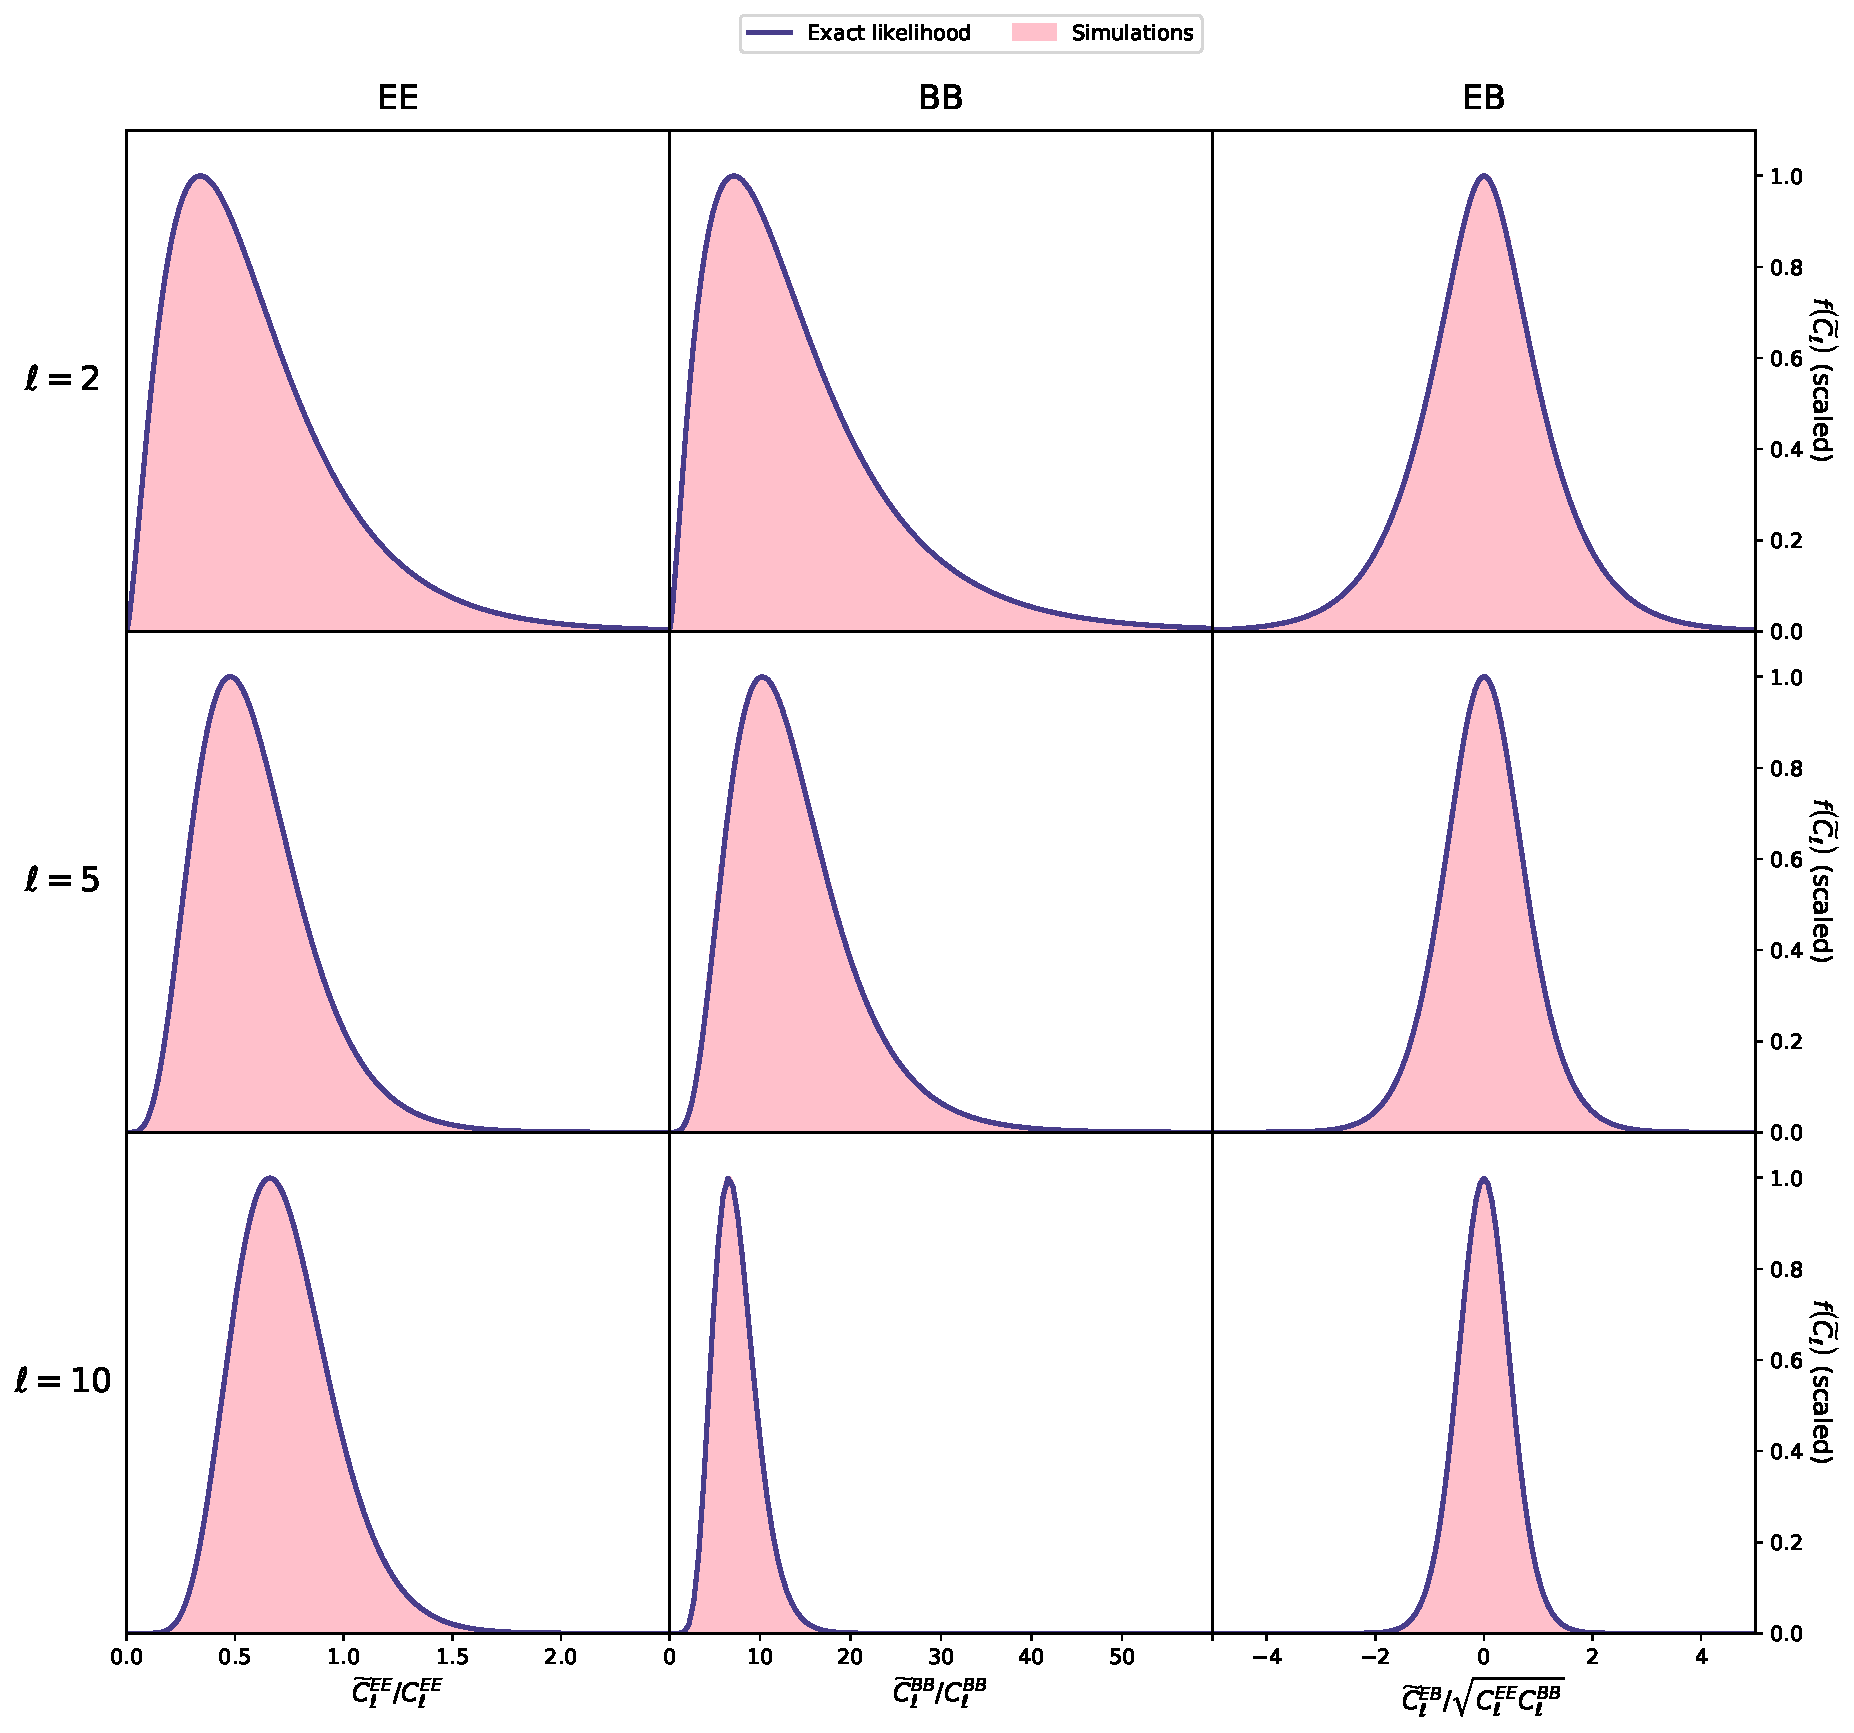
\includegraphics[width=\columnwidth]{marg_plots}
\caption{The marginal distributions of $\widetilde{C}_\ell^{EE}$, $\widetilde{C}_\ell^{BB}$ and $\widetilde{C}_\ell^{EB}$ for $\ell = 2$, 5 and 10, predicted by the exact likelihood for Gaussian fields presented in this chapter (blue curves) compared to those observed in the simulations (pink histograms). The maximum value of each curve has been rescaled to 1 for ease of comparison.}
\label{el_Fig:marginals}
\end{figure}

\autoref{el_Fig:marginals} shows the marginal distributions of $\widetilde{C}_\ell^{EE}$, $\widetilde{C}_\ell^{BB}$ and $\widetilde{C}_\ell^{EB}$ for each of $\ell = 2$, 5 and 10, to compare the prediction of the exact likelihood for Gaussian fields to the distributions observed in the simulations. Each histogram uses 300 bins. There is an excellent fit between the predicted and observed distribution, with no visible noise in the histograms due to the large number of events in each marginal distribution. The predicted likelihood exactly reproduces both the shape and amplitude of the observed distributions, including the considerable skewness in the auto-spectra. This skewness is reduced for higher multipoles, which is consistent with the full-sky behaviour of the likelihood.
Each auto-$\widetilde{C}_\ell$ in \autoref{el_Fig:marginals} has been scaled by the relevant theory $C_\ell$ used to generate both the theoretical likelihood and the simulations. In the case of the cross-spectrum $\widetilde{C}_\ell^{EB}$, there is no input $C_\ell^{EB}$ so instead $\sqrt{ C_\ell^{EE} C_\ell^{BB} }$ is used for the normalisation. This scaling allows us to observe that the $E$-mode power is reduced by the sky cut while the $B$-mode power is increased. This is a result of $E$--$B$ mixing: the $EE$ power spectrum is much larger in magnitude than the $BB$ power spectrum (by a factor $\sim 200$ at $\ell = 2$), meaning that the $E$--$B$ mixing induced by the mask leads to a relative increase in $B$-mode power at the expense of $E$-mode power.

\subsection{Correlation between spectra}

As well as exactly reproducing marginal distributions, the exact likelihood naturally describes correlations both between multipoles of the same spectrum and between spectra, for Gaussian fields. As described in \autoref{el_Sec:examples}, we formed the three-dimensional joint likelihood of $\widetilde{C}_\ell^{EE}$, $\widetilde{C}_\ell^{BB}$ and $\widetilde{C}_\ell^{EB}$ for $\ell = 2$. We formed the corresponding simulated distribution by binning events in three dimensions, using 100 bins in each dimension. We then integrated the exact likelihood over the volume of each histogram bin to allow for comparison between theory and simulations. Figures \ref{el_Fig:2D_EEBB}--\ref{el_Fig:2D_BBEB} show two-dimensional slices of this three-dimensional likelihood. Each slice corresponds to fixing a single histogram bin in one dimension and shows all bins in the other two dimensions. The exact likelihood appears to accurately match the observed distributions in all six slices to within pixel noise that arises from the finite number of realisations in the simulations. The right-hand panel for each slice shows the logarithmic fractional residual, defined as
\begin{equation}
    r = \log_{10} \left(
    \frac{\big\lvert
    \text{sampled density from simulations}
    - \text{density from exact likelihood}
    \big\rvert}{\text{density from exact likelihood}}
    \right).
    \label{el_Eqn:resid_def}
\end{equation}
Bins with no sampled events have $r = 0$ and appear as white in Figures \ref{el_Fig:2D_EEBB}--\ref{el_Fig:2D_BBEB}. These areas were not explicitly excluded, but their probability is very low (albeit non-zero). No clear evidence of structure is otherwise seen in these residuals, indicating that these bins contain only noise. This is mostly at the level of $r \approx -4$ to $-2$, except for a small number of outlying bins whose probability density is so low that the expected number of events in each bin from the 276~million simulations is significantly less than 1, leading to fractional residual values up to $r \approx 2$ in those bins in which an event was observed.

\begin{figure}
    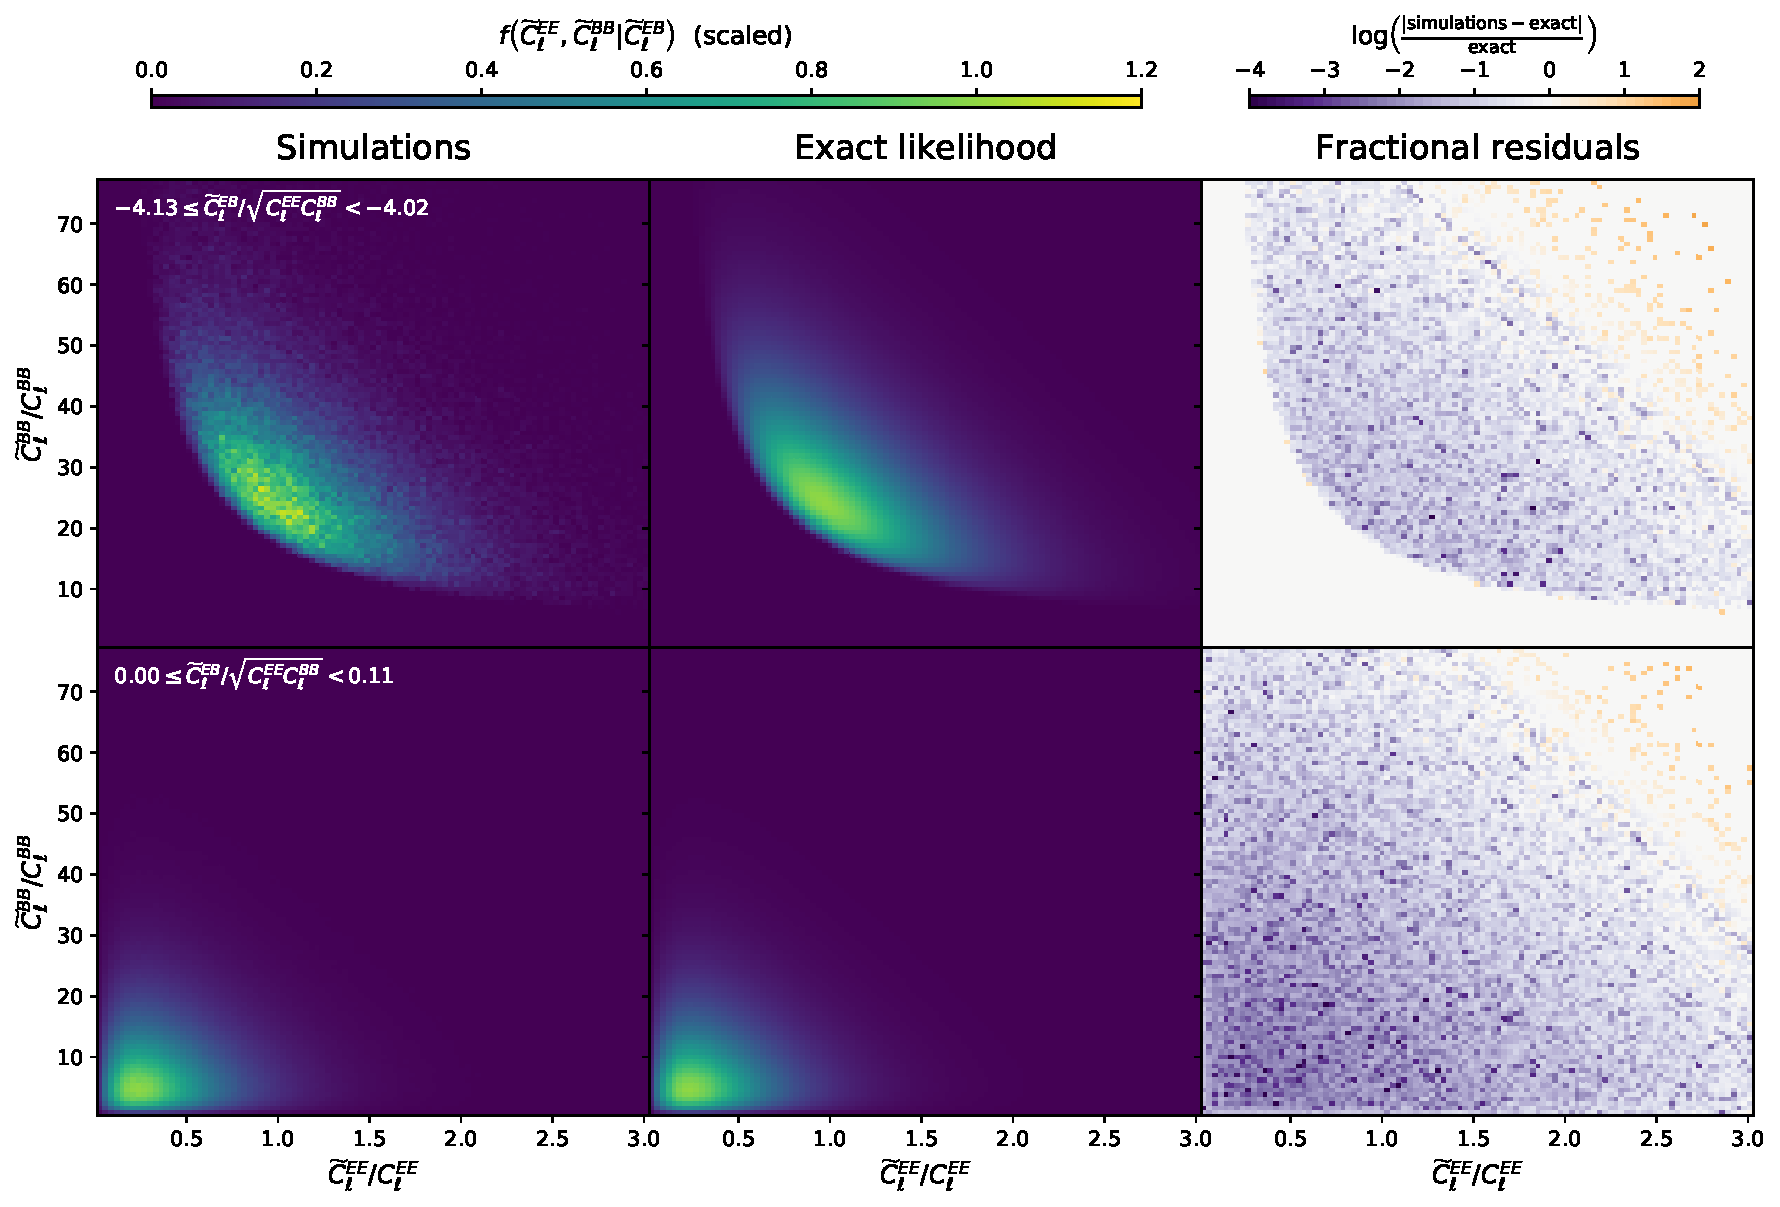
\includegraphics[width=\columnwidth]{2D_EEBB}
    \caption{Two different slices of the joint $\widetilde{C}_\ell^{EE}$--$\widetilde{C}_\ell^{BB}$ distribution for $\ell = 2$, each for one fixed bin of $\widetilde{C}_\ell^{EB}$. The top row is the slice corresponding to $-4.13~\leq~\widetilde{C}_\ell^{EB} / \sqrt{ C_\ell^{EE} C_\ell^{BB} } < -4.02$ while the bottom row corresponds to $0.00~\leq~\widetilde{C}_\ell^{EB} / \sqrt{ C_\ell^{EE} C_\ell^{BB} } < 0.11$. The left panel in each row is the distribution observed from simulations, while the centre panel is the distribution predicted by the exact likelihood for Gaussian fields. The same colour scale is used for the left and centre panels within each row and has been chosen such that the exact likelihood in each slice runs between 0 and 1. The right panels show logarithmic fractional residuals, as defined in Equation \eqref{el_Eqn:resid_def}, and contain only noise due to the finite number of realisations.}
    \label{el_Fig:2D_EEBB}
\end{figure}
\begin{figure}
    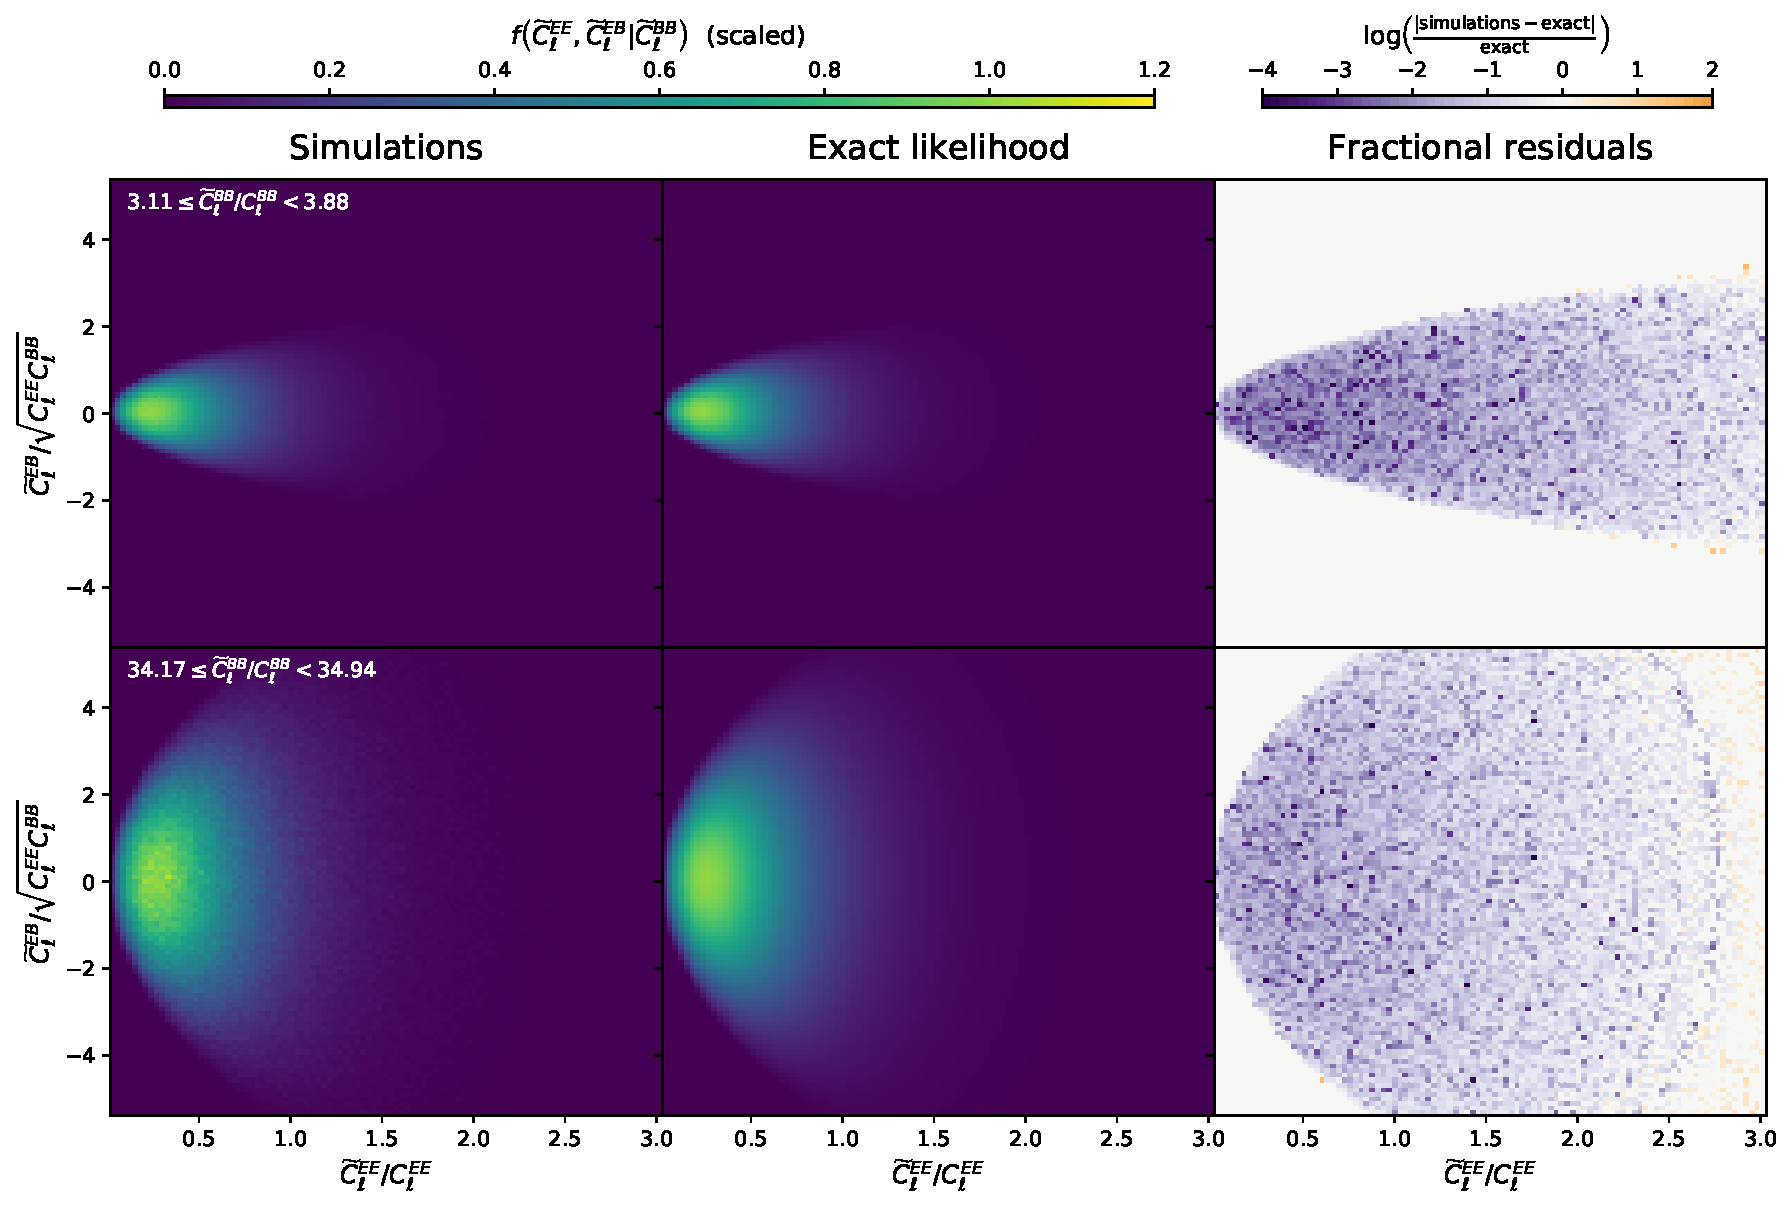
\includegraphics[width=\columnwidth]{2D_EEEB}
    \caption{As \autoref{el_Fig:2D_EEBB}, but for the $\widetilde{C}_\ell^{EE}$--$\widetilde{C}_\ell^{EB}$ distribution at fixed values of $\widetilde{C}_\ell^{BB}$. The top row corresponds to $3.11~\leq~\widetilde{C}_\ell^{BB} / C_\ell^{BB} < 3.88$ and the bottom row to $34.17~\leq~\widetilde{C}_\ell^{BB} / C_\ell^{BB} < 34.94$.}
\end{figure}
\begin{figure}
    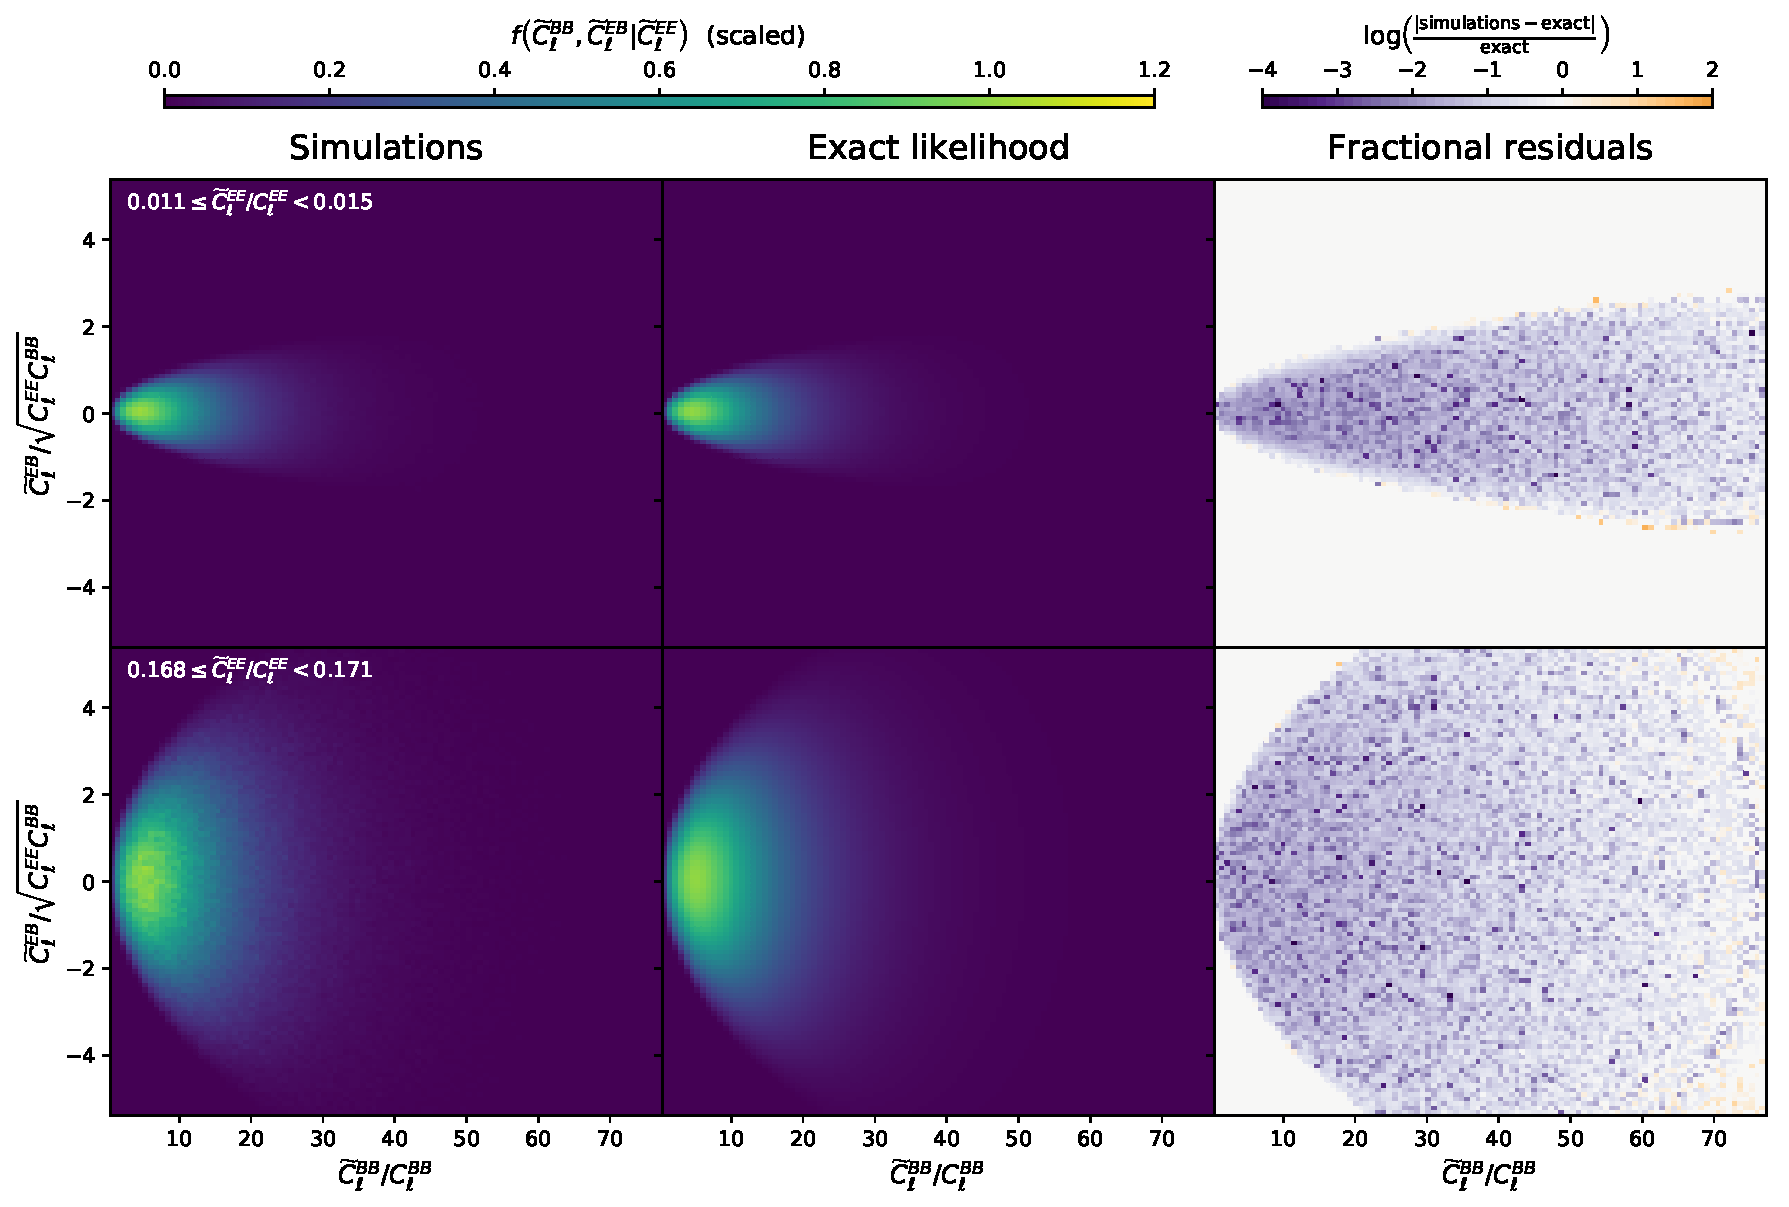
\includegraphics[width=\columnwidth]{2D_BBEB}
    \caption{As \autoref{el_Fig:2D_EEBB}, but for the $\widetilde{C}_\ell^{BB}$--$\widetilde{C}_\ell^{EB}$ distribution at fixed values of $\widetilde{C}_\ell^{EE}$. The top row corresponds to $0.011~\leq~\widetilde{C}_\ell^{EE} / C_\ell^{EE} < 0.015$ and the bottom row to $0.168~\leq~\widetilde{C}_\ell^{EE} / C_\ell^{EE} < 0.171$.}
    \label{el_Fig:2D_BBEB}
\end{figure}

\subsubsection{Comparison to approximation}

In this section, the exact likelihood is compared to a Wishart distribution with fitted parameters $\nu_\mathrm{eff}$ and $\mathbfss{W}_\ell^\mathrm{eff}$, as described in \autoref{el_Eqn:sec_approx}. This comparison is not included to advocate for the use of this approximation; on the contrary, the aim is to demonstrate the merits of using the exact likelihood for Gaussian fields. For this reason, it is not a concern whether appropriate values of $\nu_\mathrm{eff}$ and $\mathbfss{W}_\ell^\mathrm{eff}$ can be obtained in practice. We simultaneously fitted the three marginals of a $p=2$ Wishart distribution to the exact marginals, and obtained the following best-fitting values:
\begin{equation}
    \frac{\nu_\mathrm{eff}}{2 \ell + 1} = 1.0; \quad \quad
    \mathbfss{W}_\ell^\mathrm{eff} = \frac{1}{2 \ell + 1}
    \begin{pmatrix}
    0.59 C_\ell^{EE} & 0 \\
    0 & 14 C_\ell^{BB}
    \end{pmatrix}.
    \label{el_Eqn:wish_params}
\end{equation}

\begin{figure}
    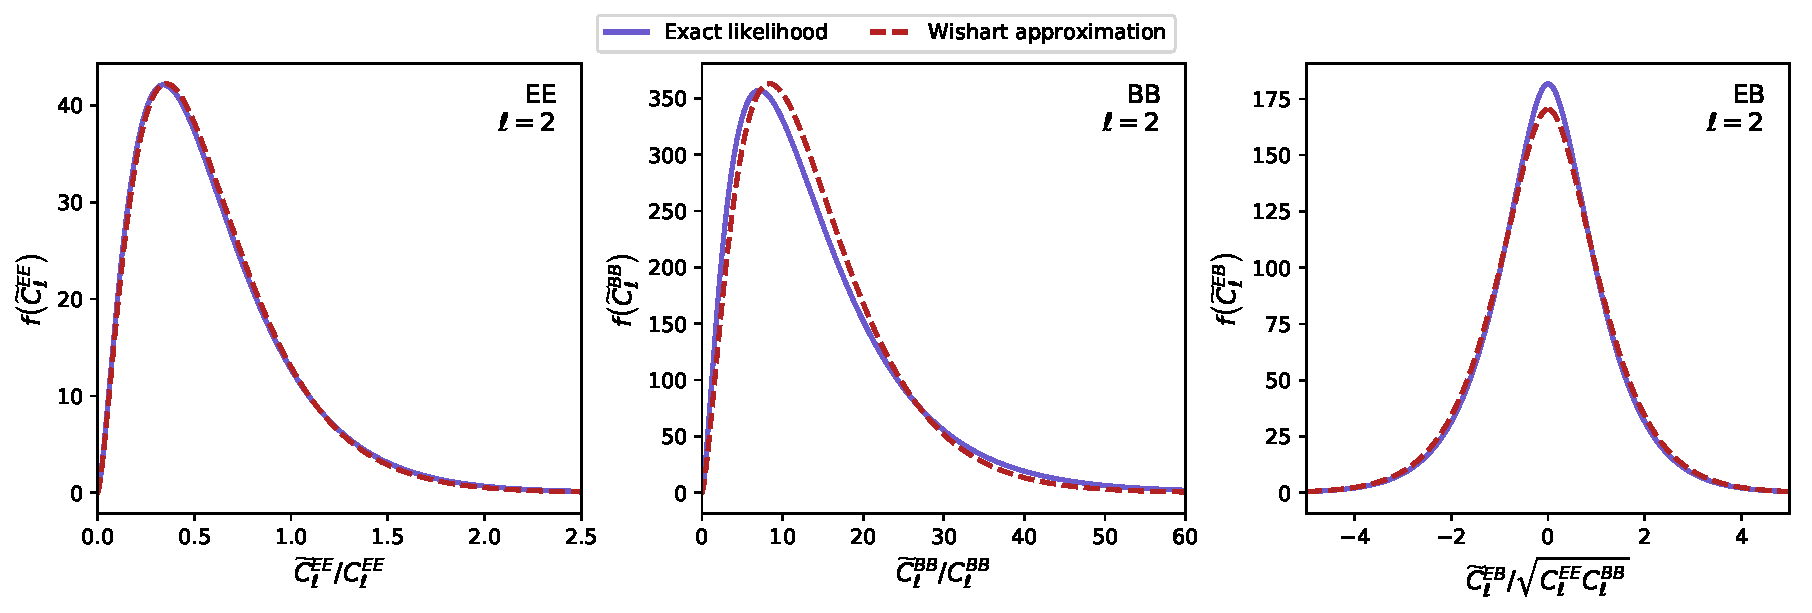
\includegraphics[width=\columnwidth]{marg_vs_approx}
    \caption{Marginal distributions based on the Wishart approximation with best-fitting parameters given in Equation \eqref{el_Eqn:wish_params} (dashed red curves) compared to the exact likelihood for Gaussian fields (solid blue curves).}
    \label{el_Fig:marg_vs_approx}
\end{figure}

There is no reason to expect that these values would also be the best-fitting values for a different $\ell$ or for a different input cosmology, and they would certainly be different for another mask. The resulting marginal distributions are shown in \autoref{el_Fig:marg_vs_approx}, where the simulated histogram is omitted for clarity. The fit is almost perfect for $\widetilde{C}_\ell^{EE}$, indicating that this marginal distribution closely follows a gamma distribution as in the full-sky case. There is slightly more deviation for $\widetilde{C}_\ell^{BB}$ and $\widetilde{C}_\ell^{EB}$.

\begin{figure}
    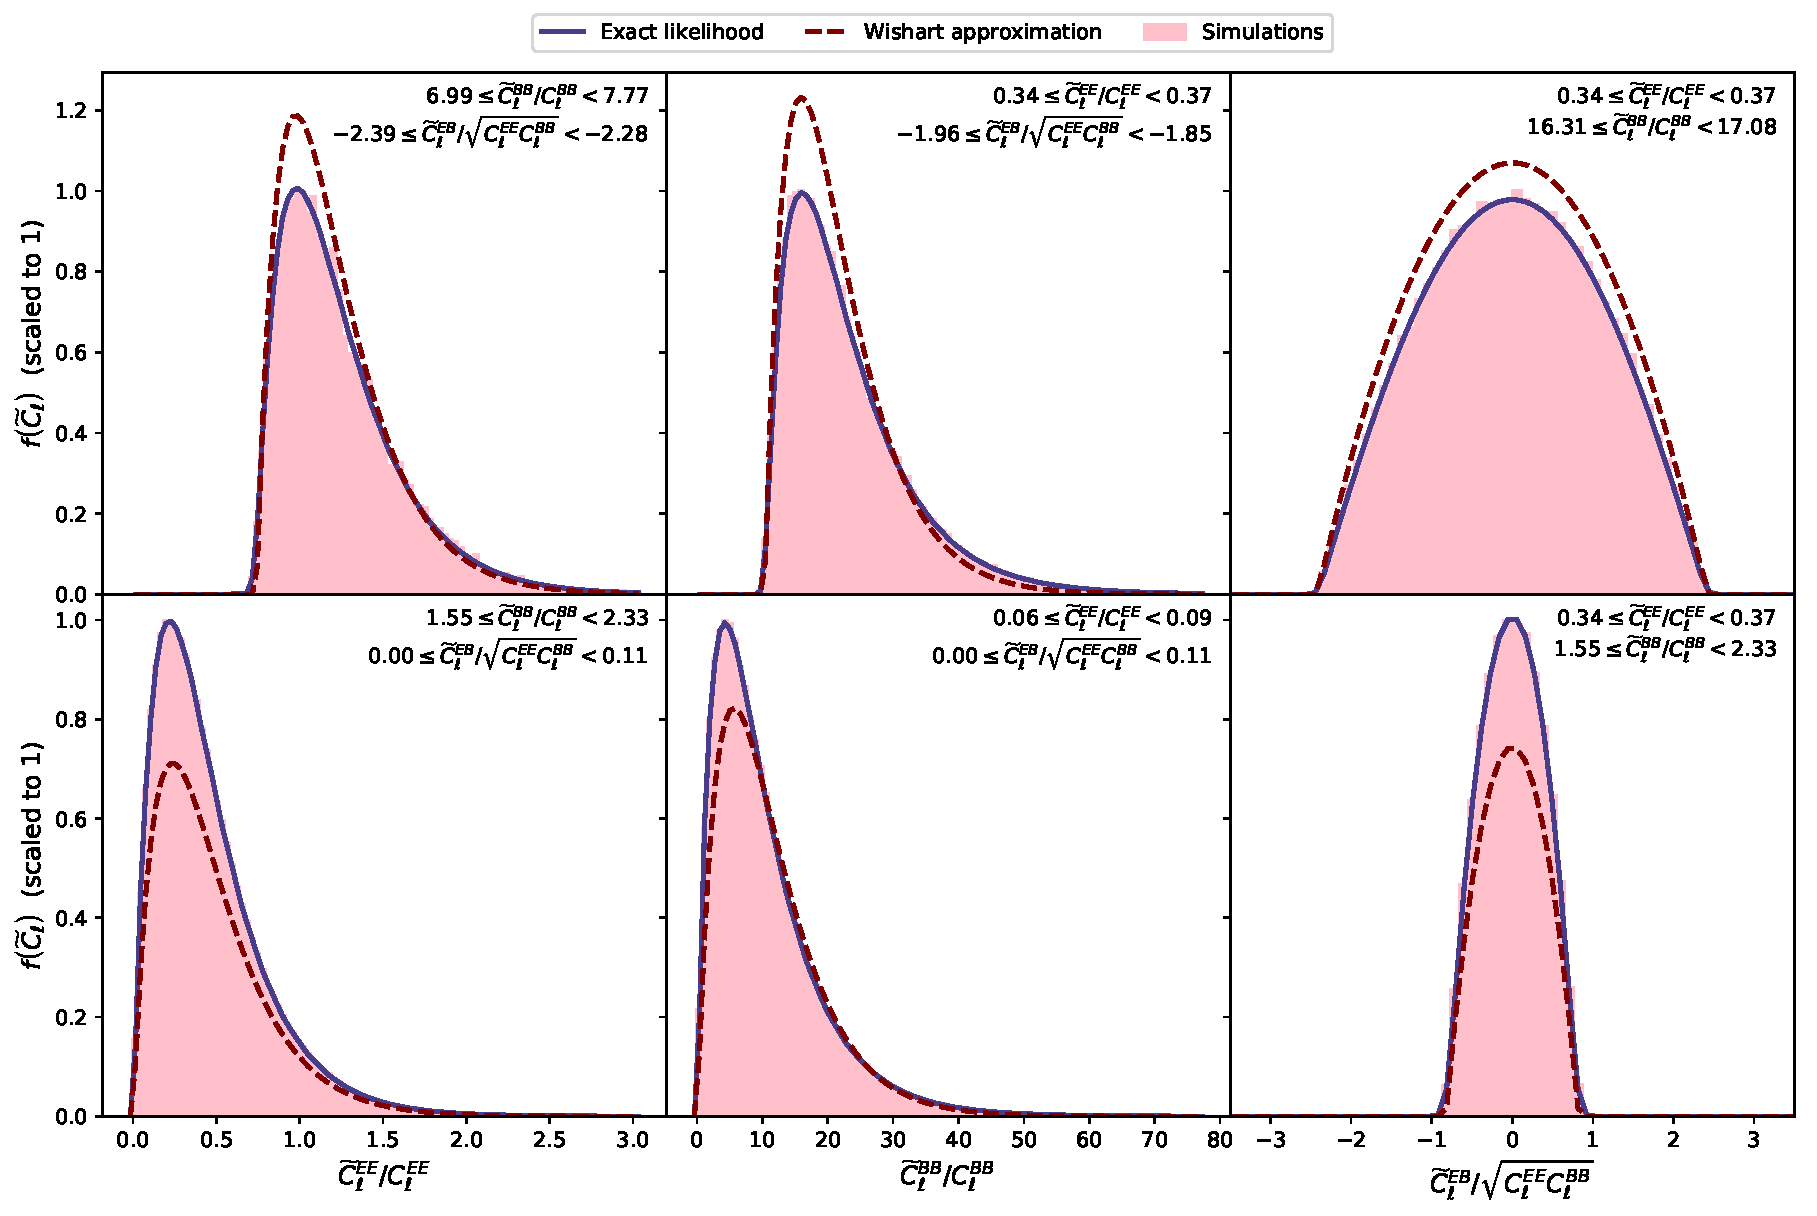
\includegraphics[width=\columnwidth]{1dslices_vs_approx}
    \caption{One-dimensional slices of the joint distribution of $\widetilde{C}_\ell^{EE}$, $\widetilde{C}_\ell^{BB}$ and $\widetilde{C}_\ell^{EB}$ for $\ell = 2$. In each slice, two of the values are fixed while the third is allowed to vary.}
    \label{el_Fig:1dslices_vs_approx}
\end{figure}

\begin{figure}
    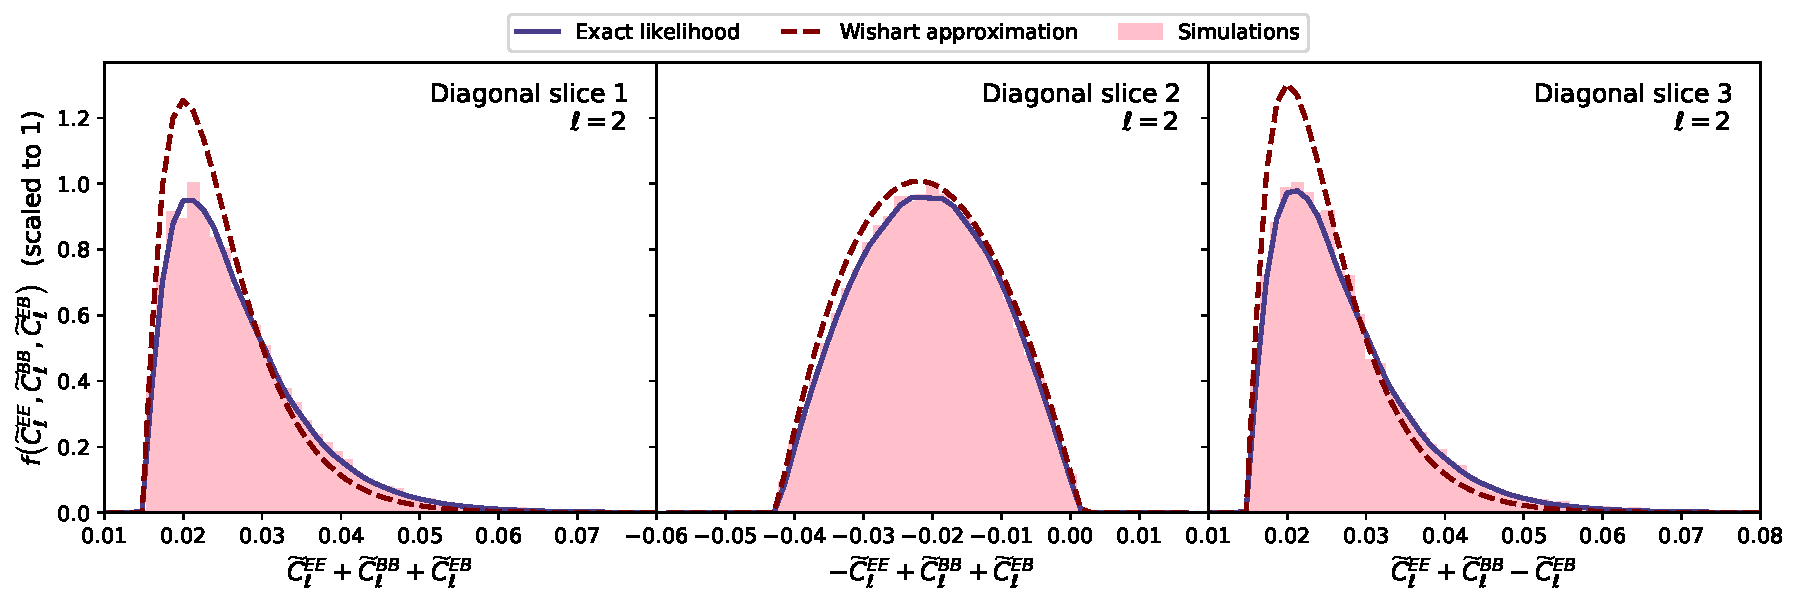
\includegraphics[width=\columnwidth]{diag_vs_approx}
    \caption{As \autoref{el_Fig:1dslices_vs_approx} but for slices taken in three diagonal directions, each corresponding to a linear combination of the three pseudo-$C_\ell$s.}
    \label{el_Fig:diag_vs_approx}
\end{figure}

We integrated the Wishart probability density over each histogram bin in three-dimensional space, as with the exact likelihood for Gaussian fields. \autoref{el_Fig:1dslices_vs_approx} shows one-dimensional slices through this three-dimensional likelihood. For each slice, two dimensions have been fixed at a single histogram bin, and the distribution across the third dimension is shown. While the marginal distributions suggest a near-exact fit for the Wishart approximation, the one-dimensional slices reveal that the approximation incorrectly distributes probability in some parts of the three-dimensional space relative to other parts. The exact likelihood for Gaussian fields, on the other hand, faithfully reproduces the observed distribution throughout. This is also seen in \autoref{el_Fig:diag_vs_approx}, which shows three one-dimensional slices in different diagonal directions across the three-dimensional space. In each of these slices, the Wishart approximation overestimates the probability density relative to the true distribution, implying that it must underestimate it in other parts of the distribution, given that the whole distribution is normalised to integrate to 1.

As well as failing to accurately reproduce the full distribution for a fixed $\ell$, the Wishart distribution cannot naturally be extended to include correlations between multipoles, whereas the exact likelihood automatically produces the full joint distribution between all multipoles of all power spectra measured on Gaussian fields. In some cases an approximation may work better over the joint distribution of many multipoles than for a single $\ell$ \citep{Hamimeche2008}, but the inverse can also be true \citep{Elsner2012}. In any case, the choice of approximation for the purposes of this comparison is unimportant: no approximation can completely match the exact distribution.


\section{Conclusions}
\label{el_Sec:conclusions}

This chapter has presented the exact joint likelihood of an arbitrary number of pseudo-$C_\ell$ estimates from correlated Gaussian fields, valid for both auto- and cross-power spectra and for any mask geometry. The likelihood---given in Equation \eqref{el_Eqn:joint_likelihood}---naturally models both intrinsic correlations between spin-0 and spin-2 fields, and correlations induced by a cut sky which result in the mixing between spherical harmonic coefficients. The pseudo-$a_{\ell m}$s follow a multivariate Gaussian distribution with covariance matrix elements given by Equations \eqref{el_Eqn:cov_re_re_general}--\eqref{el_Eqn:cov_re_im_general}. The exact joint likelihood for QML power spectrum estimates from Gaussian fields has also been presented, in Equation \eqref{el_Eqn:qml_distribution}. An accurate likelihood function is an essential companion to any estimator for unbiased cosmological inference, but until now a complete likelihood for either the pseudo-$C_\ell$ or QML estimator on an arbitrary sky has not been known.

Sections \ref{el_Sec:examples} and \ref{el_Sec:results} showed how the exact likelihood can be applied to observations of the polarisation of the Cosmic Microwave Background. This is especially relevant given current and future experiments aimed at detecting primordial $B$-modes, which require exquisite control of all possible sources of systematic bias. One such source of bias is an inexact likelihood function, so knowledge of the exact likelihood could play an important role in extracting cosmological information from polarisation measurements in an unbiased manner. In particular, it exactly models the leakage of $E$-mode power into the much smaller $B$-mode signal. This likelihood also extends naturally to include correlations between temperature anisotropy and polarisation, including cross-correlations between any number of detectors, where each observed temperature or polarisation field may have its own mask. It does not account for weak gravitational lensing of the CMB, which breaks the assumption of Gaussianity at higher multipoles.

The exact likelihood for Gaussian fields could also be extremely useful for weak lensing observations. It will perhaps be most valuable at relatively low multipoles, as this is the regime where the common assumption of a Gaussian likelihood for power spectrum estimates is least applicable due to the considerable skewness in the true likelihood \citep[e.g.][]{Sellentin2018a}. These low multipoles correspond to large physical scales, for which it is an excellent approximation to describe the spin-2 cosmic shear field as a Gaussian field. At higher multipoles there will be significant deviations from Gaussianity, so this likelihood cannot be considered exact on small scales. The likelihood naturally extends to describe the full distribution of auto- and cross-power spectra between an arbitrary number of redshift bins, each with its own mask. It is thus well suited for extracting robust cosmological constraints from tomographic galaxy clustering and weak lensing shear power spectrum measurements in multiple redshift bins, such as those from \Euclid{}.

Use of the exact pseudo-$C_\ell$ likelihood for Gaussian fields is likely to be competitive in terms of speed when considering a small number of bandpower estimates. Its main strength compared to an exact pixel-based likelihood is that for a single power estimate the pseudo-$C_\ell$ likelihood requires the determinant evaluation of a matrix of size $\sim \ell$ compared to $\sim \ell^2$ for a pixel-based method. This means that it may be evaluated at much higher $\ell$ than is possible for a pixel-based method. However, once many power estimates are considered the scaling is less competitive. The pixel-based method would offer all additional multipoles $\ell' < \ell$ without significant additional computational cost, while the exact pseudo-$C_\ell$ likelihood for Gaussian fields scales as $\sim k^N$, where $N$ is the number of (band)power estimates and $k \sim 200$. The cost is driven by the need to evaluate the characteristic function in Equation \eqref{el_Eqn:joint_cf} for every value of the vector $\mathbfit{t}$. The range of $\mathbfit{t}$ must cover a wide enough space for the integral in the likelihood expression to converge, while at a sufficiently high resolution so that its curvature is accurately represented. Each point in $\mathbfit{t}$-space carries its own determinant or eigenvalue calculation (which is not the case for a single power estimate, due to the simple scaling of the determinant of a single matrix).
% Use of the exact likelihood for Gaussian fields is therefore only recommended in the case of a small number of bandpower estimates, and are exploring alternative (necessarily approximate) approaches for the joint distribution of many power estimates, including the use of a copula with the exact marginal distributions.
Use of the exact likelihood for Gaussian fields is therefore only recommended in the case of a very small number of bandpower estimates, and alternative (necessarily approximate) approaches for the joint distribution of many power estimates should be explored. One possibility is the use of a copula with the exact marginal distributions.
Copula methods have previously been described in a cosmological context, but only with approximate marginal distributions \citep{Benabed2009, Sato2010, Sato2011}. Alternative approaches previously explored in the literature include approximate extensions to the Wishart distribution to model correlations between multipoles \citep{Hamimeche2008, Mangilli2015}. Computational limitations in the likelihood calculation may also be mitigated to some extent by potential speed increases at other levels in the inference process such as neural net-assisted sampling \citep{Manrique-Yus2020}.

Despite the limitations of its direct use, knowledge of the exact pseudo-$C_\ell$ and QML likelihood for Gaussian fields is extremely useful as a starting point and testing benchmark for developing fast, accurate approximations. It is used for this purpose in the work presented in \autoref{chap:gauss_like}. A common approach to a total likelihood, particularly for CMB observations \citep[e.g.][]{Planck2018V} is to use an exact pixel-based likelihood at low multipoles and to switch to an approximate Gaussian power spectrum likelihood for higher multipoles, at the point at which a pixel-based likelihood becomes computationally unfeasible (at $\ell = 29$ in the case of \Planck{}, while for weak lensing analyses with many redshift bins an exact pixel-based method may not be feasible at all). Methods derived from this exact likelihood for Gaussian fields may fill an important niche between these two regimes, allowing the use of an exact or near-exact likelihood up to higher multipoles than is currently possible. This may be a powerful tool for interpreting future observations, given the increased statistical precision that they will offer. This likelihood also has the advantage that it can naturally describe the cross-correlation power spectrum measured between two different maps, in contrast to exact pixel-based methods which are not readily adapted to extracting just the cross-correlation information. Considering only cross-spectra in this way makes the cosmological analysis insensitive to the details of the noise bias, which will be especially relevant for cosmic shear observations, for which shape noise is an important and uncertain factor.


% % Uncomment to build alone without subfiles:
% \printbibliography[heading=bibintoc]
% \end{document}
